\documentclass[12pt]{article}
%\usepackage{natbib}
\usepackage[numbers]{natbib}
\usepackage{amsthm}
\usepackage[toc,page]{appendix}
\usepackage{color}
\usepackage{graphicx}
\usepackage{tabularx}
\usepackage{caption}

\usepackage{longtable}
\usepackage[]{inputenc}
\usepackage[T1]{fontenc}
\usepackage{fullpage}
\usepackage{coqdoc}
\usepackage{amsmath,amssymb}
\usepackage{listings}


\DeclareGraphicsExtensions{.pdf,.png,.jpg}
\definecolor{codegreen}{rgb}{0,0.6,0}
\definecolor{codegray}{rgb}{0.5,0.5,0.5}
\definecolor{codepurple}{rgb}{0.58,0,0.82}
\definecolor{backcolour}{rgb}{0.95,0.95,0.92}

\DeclareCaptionFormat{listing}{#1#2#3}
\captionsetup[lstlisting]{format=listing,singlelinecheck=false} 

\lstdefinestyle{mystyle}{
    backgroundcolor=\color{backcolour},   
    commentstyle=\color{codegreen},
    keywordstyle=\color{magenta},
    numberstyle=\tiny\color{codegray},
    stringstyle=\color{codepurple},
    basicstyle=\footnotesize,
    breakatwhitespace=false,         
    breaklines=true,                 
    captionpos=b,                    
    keepspaces=true,                 
    numbers=left,                    
    numbersep=5pt,                  
    showspaces=false,                
    showstringspaces=false,
    showtabs=false,                  
    tabsize=2
}
\newtheorem{mydef}{Definition}


\begin{document}

\begin{appendices}
\end{appendices}
\section{Full Results - C}\label{FullResults}

\subsection{Table - DFA2 Analysis results per source file}
\begin{longtable}{l l r r r}
\textbf{Filename} & \textbf{Type} & \textbf{H} & \textbf{+/-} & \textbf{R} \\
{gnu/usr.bin/gcc/gcc/recog} & tab3 & 0.59492 & 0.0056327 & 0.99974 \\
{gnu/gcc/gcc/dbxout} & trim & 0.59263 & 0.0061208 & 0.99969 \\
{gnu/usr.bin/perl/hv} & tab8 & 0.70414 & 0.008119 & 0.99961 \\
{gnu/gcc/gcc/dbxout} & tab3 & 0.60669 & 0.0069868 & 0.99961 \\
{gnu/usr.bin/gcc/gcc/recog} & tab8 & 0.6277 & 0.0072911 & 0.9996 \\
{gnu/gcc/gcc/dbxout} & naive & 0.59439 & 0.0069626 & 0.9996 \\
{gnu/usr.bin/gcc/gcc/recog} & trim & 0.58905 & 0.0073385 & 0.99954 \\
{sys/dev/ic/mpi} & tab8 & 0.63435 & 0.0079974 & 0.99953 \\
{sys/dev/ic/mpi} & tab3 & 0.65327 & 0.0082775 & 0.99953 \\
{gnu/gcc/gcc/recog} & trim & 0.59532 & 0.0075579 & 0.99953 \\
{gnu/usr.bin/gcc/gcc/recog} & naive & 0.5966 & 0.0079926 & 0.99947 \\
{gnu/usr.bin/perl/hv} & tab3 & 0.69224 & 0.0097339 & 0.99942 \\
{sys/dev/pci/if/san/xilinx} & tab3 & 0.59175 & 0.0087195 & 0.99936 \\
{usr.sbin/bgpd/rde} & naive & 0.61891 & 0.0097795 & 0.99927 \\
{gnu/usr.bin/gcc/gcc/java/expr} & tab3 & 0.63189 & 0.010224 & 0.99923 \\
{usr.sbin/bgpd/rde} & trim & 0.59715 & 0.0099081 & 0.99919 \\
{sys/dev/ic/mpi} & naive & 0.66608 & 0.011323 & 0.99915 \\
{gnu/gcc/gcc/recog} & naive & 0.59523 & 0.010179 & 0.99914 \\
{sys/dev/audio} & tab3 & 0.59244 & 0.010359 & 0.9991 \\
{sys/dev/pci/if/san/xilinx} & naive & 0.56351 & 0.0098886 & 0.99909 \\
{gnu/usr.bin/perl/hv} & naive & 0.69928 & 0.012633 & 0.99904 \\
{sys/dev/ic/mpi} & trim & 0.65627 & 0.011851 & 0.99904 \\
{gnu/usr.bin/gcc/gcc/java/expr} & naive & 0.62566 & 0.01174 & 0.99896 \\
{sys/dev/audio} & tab8 & 0.64505 & 0.012165 & 0.99895 \\
{gnu/gcc/gcc/recog} & tab3 & 0.58913 & 0.011115 & 0.99895 \\
{sys/dev/pci/if/san/xilinx} & trim & 0.56666 & 0.010914 & 0.99891 \\
{gnu/gcc/gcc/dbxout} & tab8 & 0.66126 & 0.01297 & 0.99887 \\
{sys/dev/audio} & trim & 0.58605 & 0.011504 & 0.99887 \\
{sys/arch/arm/arm/pmap7} & tab8 & 0.66145 & 0.013067 & 0.99885 \\
{usr.sbin/bgpd/rde} & tab3 & 0.66746 & 0.013262 & 0.99884 \\
{gnu/usr.bin/gcc/gcc/java/expr} & tab8 & 0.65126 & 0.013331 & 0.99877 \\
{gnu/usr.bin/gcc/gcc/config/mcore/mcore} & trim & 0.66775 & 0.013741 & 0.99875 \\
{gnu/usr.bin/gcc/gcc/config/mcore/mcore} & naive & 0.67327 & 0.013939 & 0.99874 \\
{usr.sbin/bgpd/rde} & tab8 & 0.76232 & 0.016056 & 0.9987 \\
{gnu/usr.bin/gcc/gcc/config/mcore/mcore} & tab3 & 0.67179 & 0.014159 & 0.99869 \\
{gnu/gcc/gcc/config/cris/cris} & trim & 0.58868 & 0.012673 & 0.99864 \\
{sys/dev/audio} & naive & 0.58739 & 0.012703 & 0.99862 \\
{gnu/gcc/gcc/recog} & tab8 & 0.619 & 0.013698 & 0.99856 \\
{gnu/usr.bin/perl/hv} & trim & 0.67169 & 0.014941 & 0.99855 \\
{sys/dev/pci/if/oce} & tab8 & 0.65203 & 0.014539 & 0.99854 \\
{gnu/usr.bin/gcc/gcc/config/mcore/mcore} & tab8 & 0.68192 & 0.015549 & 0.99847 \\
{gnu/usr.bin/binutils-2.17/binutils/dlltool} & tab8 & 0.70437 & 0.016121 & 0.99846 \\
{gnu/usr.bin/gcc/gcc/java/expr} & trim & 0.6216 & 0.014288 & 0.99845 \\
{sys/dev/pci/if/san/xilinx} & tab8 & 0.69829 & 0.016051 & 0.99845 \\
{gnu/usr.bin/gcc/gcc/config/d30v/d30v} & tab8 & 0.6478 & 0.016048 & 0.9982 \\
{sys/arch/arm/arm/pmap7} & tab3 & 0.60489 & 0.01537 & 0.9981 \\
{gnu/usr.bin/binutils-2.17/binutils/dlltool} & tab3 & 0.67957 & 0.019866 & 0.99749 \\
{lib/libpcap/gencode} & trim & 0.68244 & 0.021502 & 0.99709 \\
{lib/libpcap/gencode} & naive & 0.68849 & 0.021903 & 0.99703 \\
{gnu/usr.bin/binutils-2.17/binutils/dlltool} & naive & 0.67264 & 0.021469 & 0.99701 \\
{gnu/gcc/gcc/config/cris/cris} & naive & 0.58113 & 0.018732 & 0.99695 \\
{lib/libpcap/gencode} & tab3 & 0.70019 & 0.022772 & 0.9969 \\
{sys/arch/arm/arm/pmap7} & trim & 0.59658 & 0.019706 & 0.9968 \\
{sys/arch/arm/arm/pmap7} & naive & 0.5988 & 0.019811 & 0.99679 \\
{gnu/usr.bin/binutils-2.17/bfd/elf32-s390} & naive & 0.73052 & 0.02483 & 0.99661 \\
{gnu/usr.bin/binutils-2.17/bfd/elf32-s390} & trim & 0.73983 & 0.0262 & 0.99632 \\
{lib/libpcap/gencode} & tab8 & 0.74311 & 0.026836 & 0.99618 \\
{gnu/usr.bin/binutils-2.17/bfd/elf32-s390} & tab3 & 0.73373 & 0.026766 & 0.9961 \\
{gnu/usr.bin/binutils-2.17/opcodes/xc16x-desc} & trim & 0.82248 & 0.030216 & 0.99605 \\
{gnu/usr.bin/binutils-2.17/opcodes/xc16x-desc} & naive & 0.80899 & 0.029991 & 0.99597 \\
{gnu/usr.bin/binutils-2.17/opcodes/xc16x-desc} & tab3 & 0.80899 & 0.029991 & 0.99597 \\
{gnu/usr.bin/binutils-2.17/opcodes/xc16x-desc} & tab8 & 0.80899 & 0.029991 & 0.99597 \\
{gnu/usr.bin/binutils-2.17/binutils/dlltool} & trim & 0.67617 & 0.0254 & 0.99587 \\
{gnu/usr.bin/binutils/gas/config/tc-sh64} & trim & 0.6629 & 0.024982 & 0.99584 \\
{sys/dev/isa/gus} & tab8 & 0.74148 & 0.028409 & 0.9957 \\
{gnu/usr.bin/binutils-2.17/gas/config/tc-sh64} & trim & 0.66133 & 0.025382 & 0.99569 \\
{gnu/gcc/gcc/config/cris/cris} & tab3 & 0.5934 & 0.023363 & 0.99546 \\
{gnu/usr.bin/binutils-2.17/bfd/elf32-s390} & tab8 & 0.75431 & 0.031066 & 0.99504 \\
{usr.sbin/nginx/src/http/modules/module} & naive & 0.63568 & 0.026926 & 0.99475 \\
{usr.sbin/nginx/src/http/modules/module} & tab3 & 0.63568 & 0.026926 & 0.99475 \\
{usr.sbin/nginx/src/http/modules/module} & tab8 & 0.63568 & 0.026926 & 0.99475 \\
{gnu/usr.bin/binutils/gas/config/tc-sh64} & naive & 0.66906 & 0.028396 & 0.99473 \\
{gnu/usr.bin/binutils/gas/config/tc-sh64} & tab8 & 0.74488 & 0.031736 & 0.99469 \\
{sys/dev/pci/if/oce} & tab3 & 0.65598 & 0.028076 & 0.99465 \\
{gnu/usr.bin/binutils-2.17/gas/config/tc-sh64} & naive & 0.66763 & 0.028806 & 0.99456 \\
{gnu/usr.bin/binutils-2.17/gas/config/tc-sh64} & tab8 & 0.74279 & 0.032291 & 0.99448 \\
{gnu/usr.bin/gcc/gcc/config/d30v/d30v} & tab3 & 0.60473 & 0.026897 & 0.99422 \\
{gnu/usr.bin/binutils/binutils/rcparse} & tab8 & 0.80088 & 0.035676 & 0.9942 \\
{gnu/usr.bin/binutils/gas/config/tc-sh64} & tab3 & 0.68449 & 0.031632 & 0.99377 \\
{gnu/gcc/gcc/cp/decl2} & tab8 & 0.65354 & 0.030368 & 0.9937 \\
{gnu/usr.bin/binutils-2.17/gas/config/tc-sh64} & tab3 & 0.68297 & 0.032151 & 0.99353 \\
{gnu/gcc/gcc/config/cris/cris} & tab8 & 0.64966 & 0.030884 & 0.99341 \\
{sys/dev/isa/gus} & tab3 & 0.71938 & 0.034781 & 0.99318 \\
{gnu/usr.bin/gcc/gcc/config/d30v/d30v} & trim & 0.62112 & 0.030845 & 0.99281 \\
{gnu/gcc/gcc/cp/decl2} & naive & 0.63327 & 0.031792 & 0.99265 \\
{gnu/gcc/gcc/cp/decl2} & tab3 & 0.63641 & 0.032096 & 0.99259 \\
{gnu/gcc/gcc/cp/decl2} & trim & 0.63474 & 0.032774 & 0.99223 \\
{sys/dev/isa/gus} & naive & 0.71854 & 0.037617 & 0.99202 \\
{usr.sbin/nginx/src/http/modules/module} & trim & 0.6735 & 0.035662 & 0.99184 \\
{sys/dev/pci/if/oce} & naive & 0.67102 & 0.036174 & 0.99154 \\
{gnu/usr.bin/gcc/gcc/config/d30v/d30v} & naive & 0.60422 & 0.032721 & 0.99147 \\
{sys/dev/isa/gus} & trim & 0.71694 & 0.03908 & 0.99136 \\
{sys/dev/pci/if/oce} & trim & 0.67623 & 0.039136 & 0.99027 \\
{gnu/usr.bin/binutils/binutils/rcparse} & tab3 & 0.82709 & 0.048396 & 0.99006 \\
{gnu/usr.bin/binutils/binutils/rcparse} & trim & 0.82182 & 0.051147 & 0.98878 \\
{gnu/usr.bin/binutils/binutils/rcparse} & naive & 0.83862 & 0.052436 & 0.98867 \\
\end{longtable}

\newpage
\subsection{Table - DFA2 Variance}\label{FullResultsVariance}

\begin{longtable}{l r}
\textbf{Filename} &  \textbf{H} \\
{gnu/gcc/gcc/config/cris/cris} & 0.06852999999999998  \\
{gnu/gcc/gcc/cp/decl2} & 0.02027000000000001  \\
{gnu/gcc/gcc/dbxout} & 0.06862999999999997  \\
{gnu/gcc/gcc/recog} & 0.029869999999999952  \\
{gnu/usr.bin/binutils-2.17/bfd/elf32-s390} & 0.02379000000000009  \\
{gnu/usr.bin/binutils-2.17/binutils/dlltool} & 0.031730000000000036  \\
{gnu/usr.bin/binutils-2.17/gas/config/tc-sh64} & 0.08145999999999998  \\
{gnu/usr.bin/binutils-2.17/opcodes/xc16x-desc} & 0.013490000000000002  \\
{gnu/usr.bin/binutils/binutils/rcparse} & 0.037739999999999996  \\
{gnu/usr.bin/binutils/gas/config/tc-sh64} & 0.08197999999999994  \\
{gnu/usr.bin/gcc/gcc/config/d30v/d30v} & 0.04358000000000006  \\
{gnu/usr.bin/gcc/gcc/config/mcore/mcore} & 0.014170000000000016  \\
{gnu/usr.bin/gcc/gcc/java/expr} & 0.02965999999999991  \\
{gnu/usr.bin/gcc/gcc/recog} & 0.03865000000000007  \\
{gnu/usr.bin/perl/hv} & 0.03244999999999998  \\
{lib/libpcap/gencode} & 0.06067  \\
{sys/arch/arm/arm/pmap7} & 0.06486999999999998  \\
{sys/dev/audio} & 0.05900000000000005  \\
{sys/dev/ic/mpi} & 0.031730000000000036  \\
{sys/dev/isa/gus} & 0.024540000000000006  \\
{sys/dev/pci/if/oce} & 0.0242  \\
{sys/dev/pci/if/san/xilinx} & 0.13478  \\
{usr.sbin/bgpd/rde} & 0.16517000000000004  \\
{usr.sbin/nginx/src/http/modules/ngx/http/mp4/module} & 0.037819999999999965  \\
\end{longtable}
\begin{longtable}{l r}
\textbf{Filename} &  \textbf{+/-} \\
{gnu/gcc/gcc/config/cris/cris} & 0.018211  \\
{gnu/gcc/gcc/cp/decl2} & 0.0024059999999999984  \\
{gnu/gcc/gcc/dbxout} & 0.006849200000000001  \\
{gnu/gcc/gcc/recog} & 0.0061401  \\
{gnu/usr.bin/binutils-2.17/bfd/elf32-s390} & 0.0062359999999999985  \\
{gnu/usr.bin/binutils-2.17/binutils/dlltool} & 0.009278999999999999  \\
{gnu/usr.bin/binutils-2.17/gas/config/tc-sh64} & 0.006909000000000002  \\
{gnu/usr.bin/binutils-2.17/opcodes/xc16x-desc} & 0.0002249999999999995  \\
{gnu/usr.bin/binutils/binutils/rcparse} & 0.016760000000000004  \\
{gnu/usr.bin/binutils/gas/config/tc-sh64} & 0.006754  \\
{gnu/usr.bin/gcc/gcc/config/d30v/d30v} & 0.016673  \\
{gnu/usr.bin/gcc/gcc/config/mcore/mcore} & 0.0018080000000000006  \\
{gnu/usr.bin/gcc/gcc/java/expr} & 0.004064  \\
{gnu/usr.bin/gcc/gcc/recog} & 0.0023599000000000007  \\
{gnu/usr.bin/perl/hv} & 0.006822  \\
{lib/libpcap/gencode} & 0.0053339999999999985  \\
{sys/arch/arm/arm/pmap7} & 0.006743999999999998  \\
{sys/dev/audio} & 0.0023440000000000006  \\
{sys/dev/ic/mpi} & 0.0038536000000000004  \\
{sys/dev/isa/gus} & 0.010670999999999996  \\
{sys/dev/pci/if/oce} & 0.024596999999999997  \\
{sys/dev/pci/if/san/xilinx} & 0.0073314999999999995  \\
{usr.sbin/bgpd/rde} & 0.006276500000000001  \\
{usr.sbin/nginx/src/http/modules/ngx/http/mp4/module} & 0.008736  \\
\end{longtable}
\begin{longtable}{l r}
\textbf{Filename} &  \textbf{R} \\
{gnu/gcc/gcc/config/cris/cris} & 0.005229999999999957  \\
{gnu/gcc/gcc/cp/decl2} & 0.0014700000000000824  \\
{gnu/gcc/gcc/dbxout} & 0.0008199999999999319  \\
{gnu/gcc/gcc/recog} & 0.0009700000000000264  \\
{gnu/usr.bin/binutils-2.17/bfd/elf32-s390} & 0.0015699999999999603  \\
{gnu/usr.bin/binutils-2.17/binutils/dlltool} & 0.002589999999999981  \\
{gnu/usr.bin/binutils-2.17/gas/config/tc-sh64} & 0.0021599999999999397  \\
{gnu/usr.bin/binutils-2.17/opcodes/xc16x-desc} & 7.999999999996898e-05  \\
{gnu/usr.bin/binutils/binutils/rcparse} & 0.005529999999999924  \\
{gnu/usr.bin/binutils/gas/config/tc-sh64} & 0.0020699999999999052  \\
{gnu/usr.bin/gcc/gcc/config/d30v/d30v} & 0.006730000000000014  \\
{gnu/usr.bin/gcc/gcc/config/mcore/mcore} & 0.000280000000000058  \\
{gnu/usr.bin/gcc/gcc/java/expr} & 0.0007800000000000029  \\
{gnu/usr.bin/gcc/gcc/recog} & 0.00026999999999999247  \\
{gnu/usr.bin/perl/hv} & 0.0010599999999999499  \\
{lib/libpcap/gencode} & 0.0009100000000000774  \\
{sys/arch/arm/arm/pmap7} & 0.0020600000000000618  \\
{sys/dev/audio} & 0.00048000000000003595  \\
{sys/dev/ic/mpi} & 0.0004899999999999904  \\
{sys/dev/isa/gus} & 0.0043400000000000105  \\
{sys/dev/pci/if/oce} & 0.00827  \\
{sys/dev/pci/if/san/xilinx} & 0.0009100000000000774  \\
{usr.sbin/bgpd/rde} & 0.0005699999999999594  \\
{usr.sbin/nginx/src/http/modules/ngx/http/mp4/module} & 0.002909999999999968  \\
\end{longtable}

\newpage
\subsection{Graphs}
\begin{center}
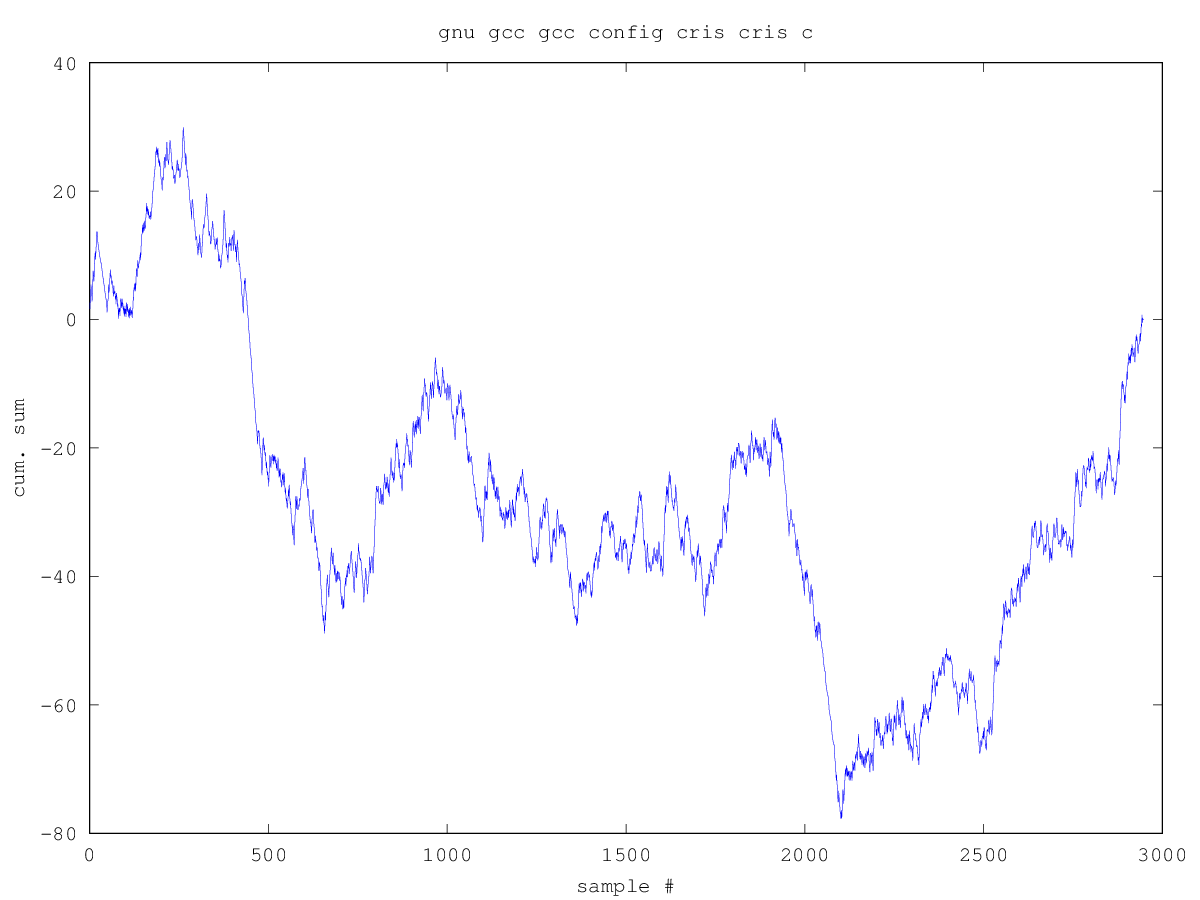
\includegraphics[width=0.8\linewidth]{{fractals/data/gnu_gcc_gcc_config_cris_cris_c_naive_time_series}.png}
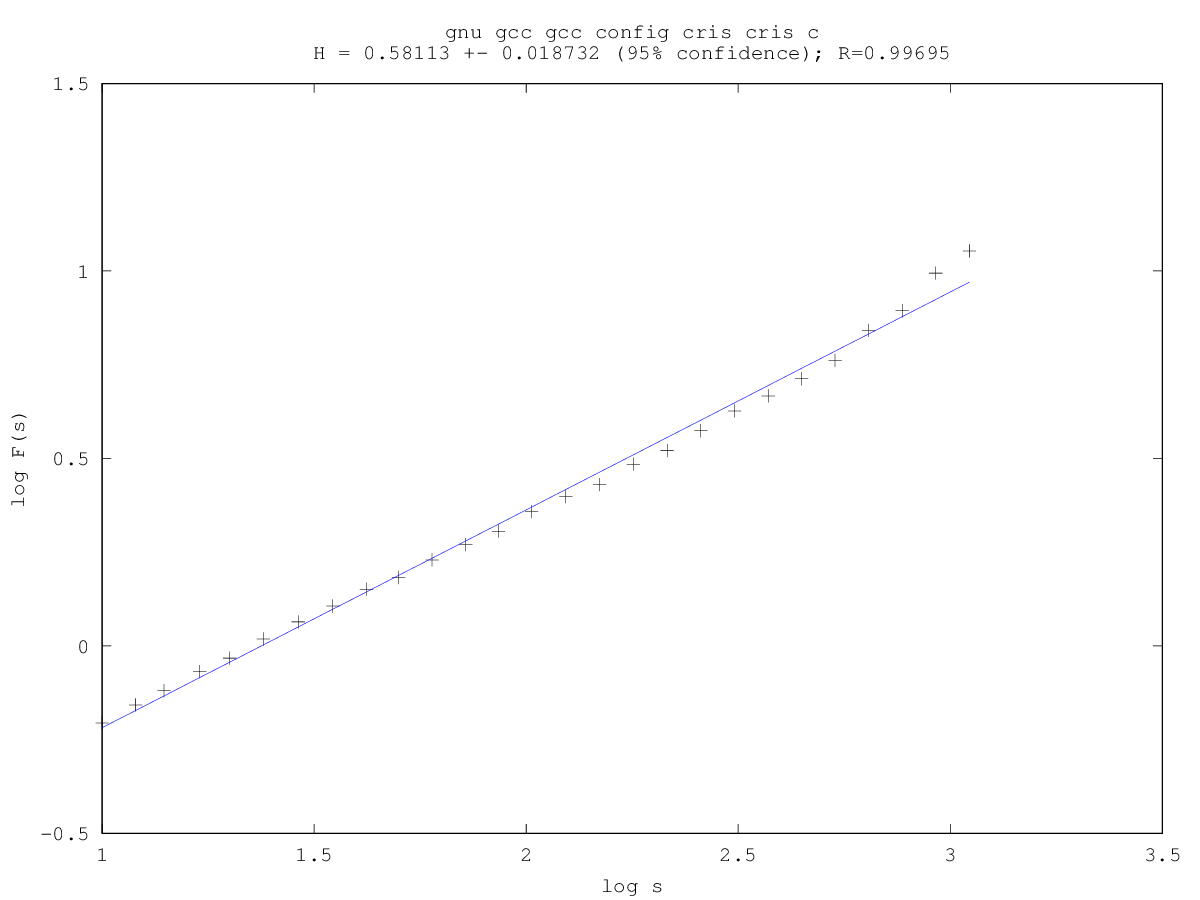
\includegraphics[width=0.8\linewidth]{{fractals/data/gnu_gcc_gcc_config_cris_cris_c_naive_log_log}.png}
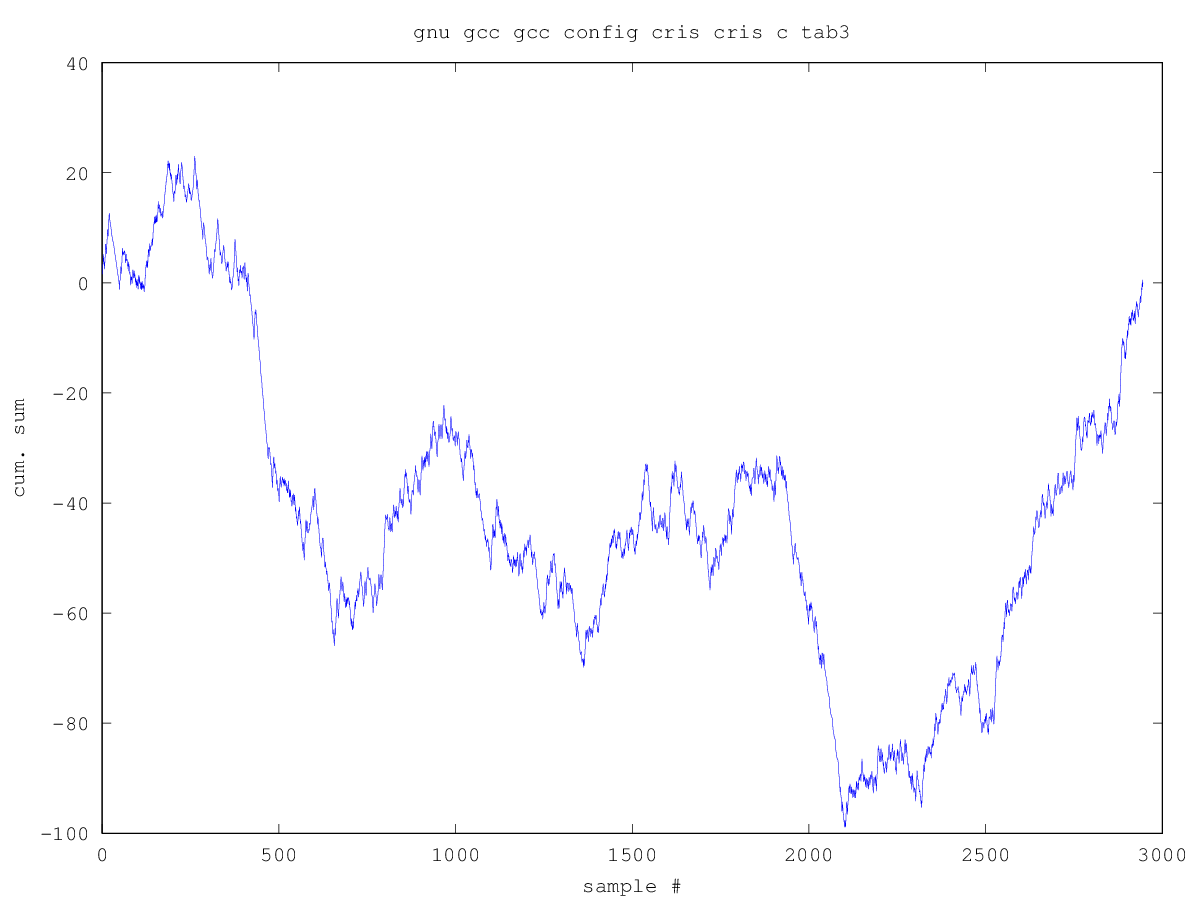
\includegraphics[width=0.8\linewidth]{{fractals/data/gnu_gcc_gcc_config_cris_cris_c_tab3_time_series}.png}
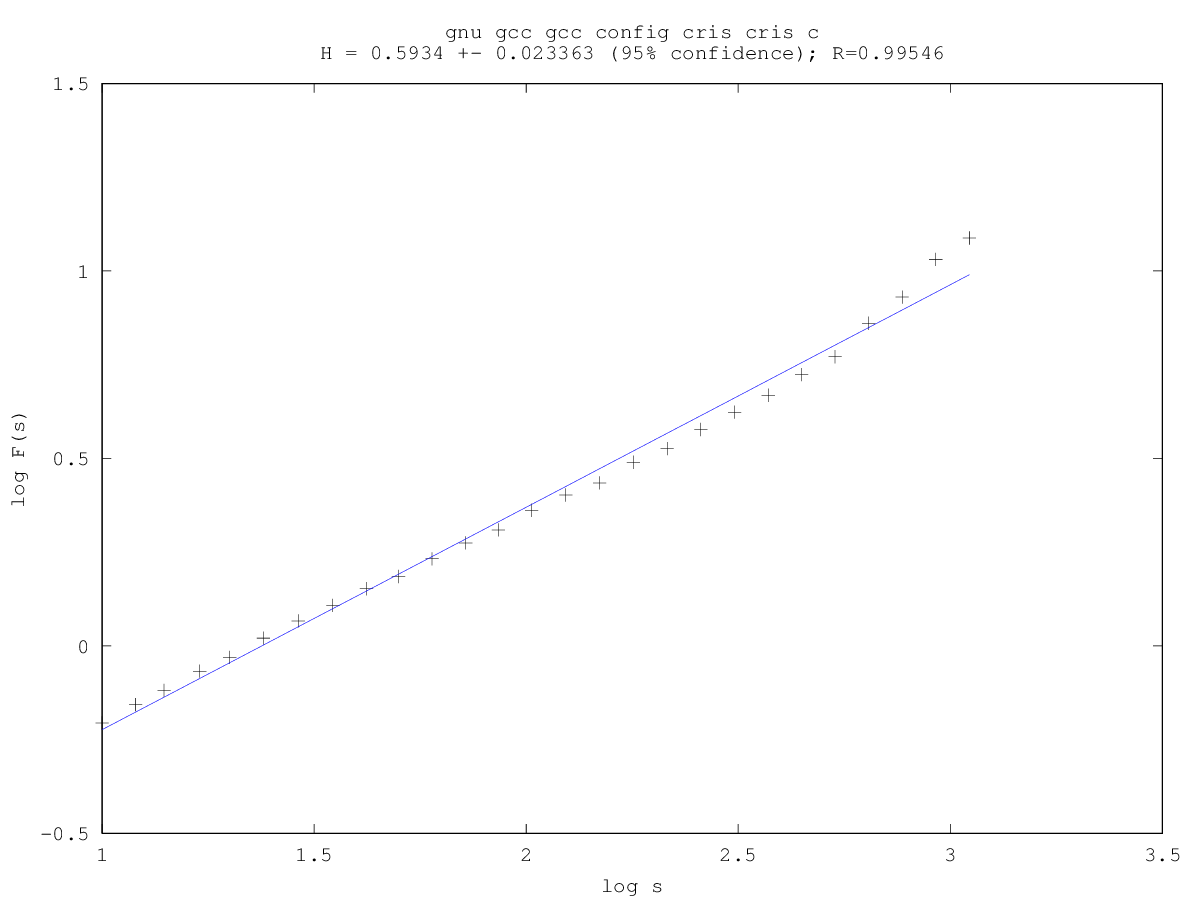
\includegraphics[width=0.8\linewidth]{{fractals/data/gnu_gcc_gcc_config_cris_cris_c_tab3_log_log}.png}
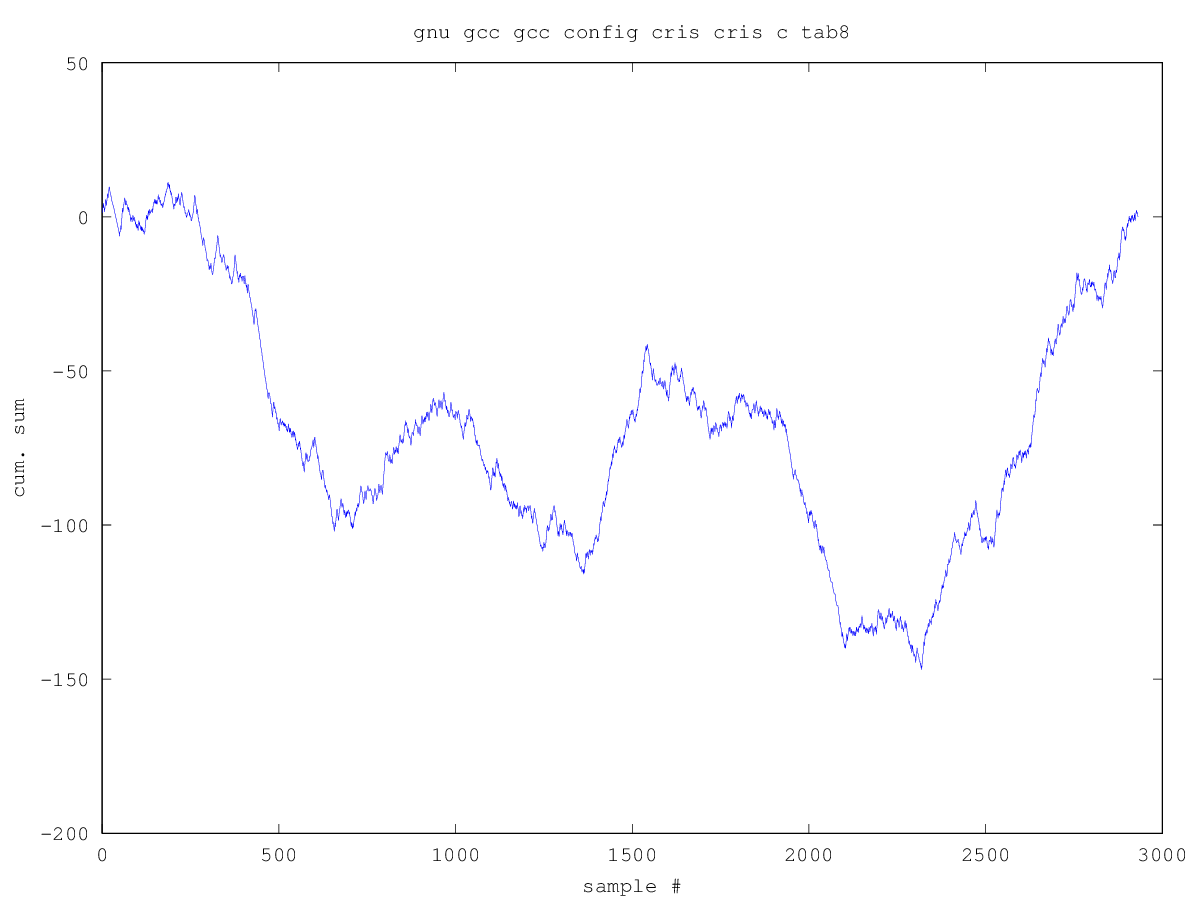
\includegraphics[width=0.8\linewidth]{{fractals/data/gnu_gcc_gcc_config_cris_cris_c_tab8_time_series}.png}
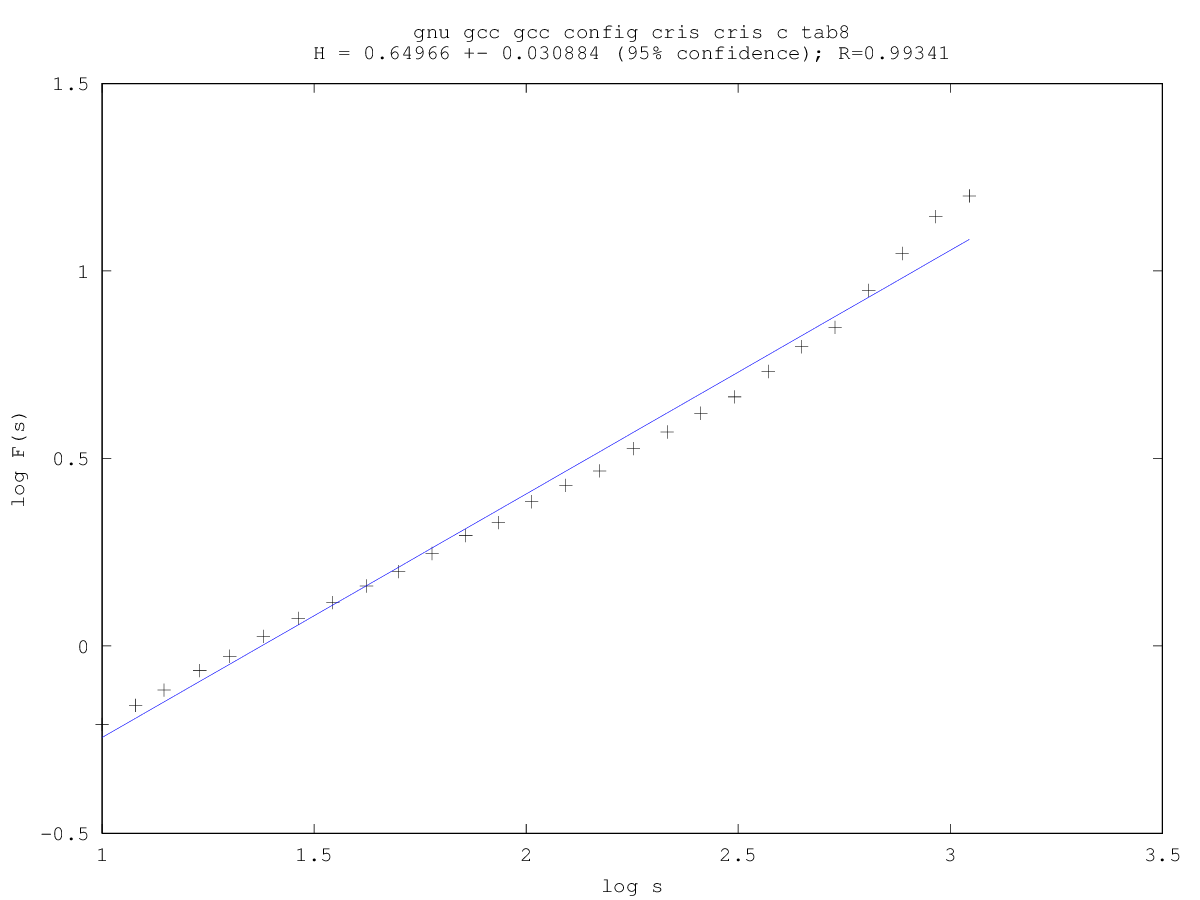
\includegraphics[width=0.8\linewidth]{{fractals/data/gnu_gcc_gcc_config_cris_cris_c_tab8_log_log}.png}
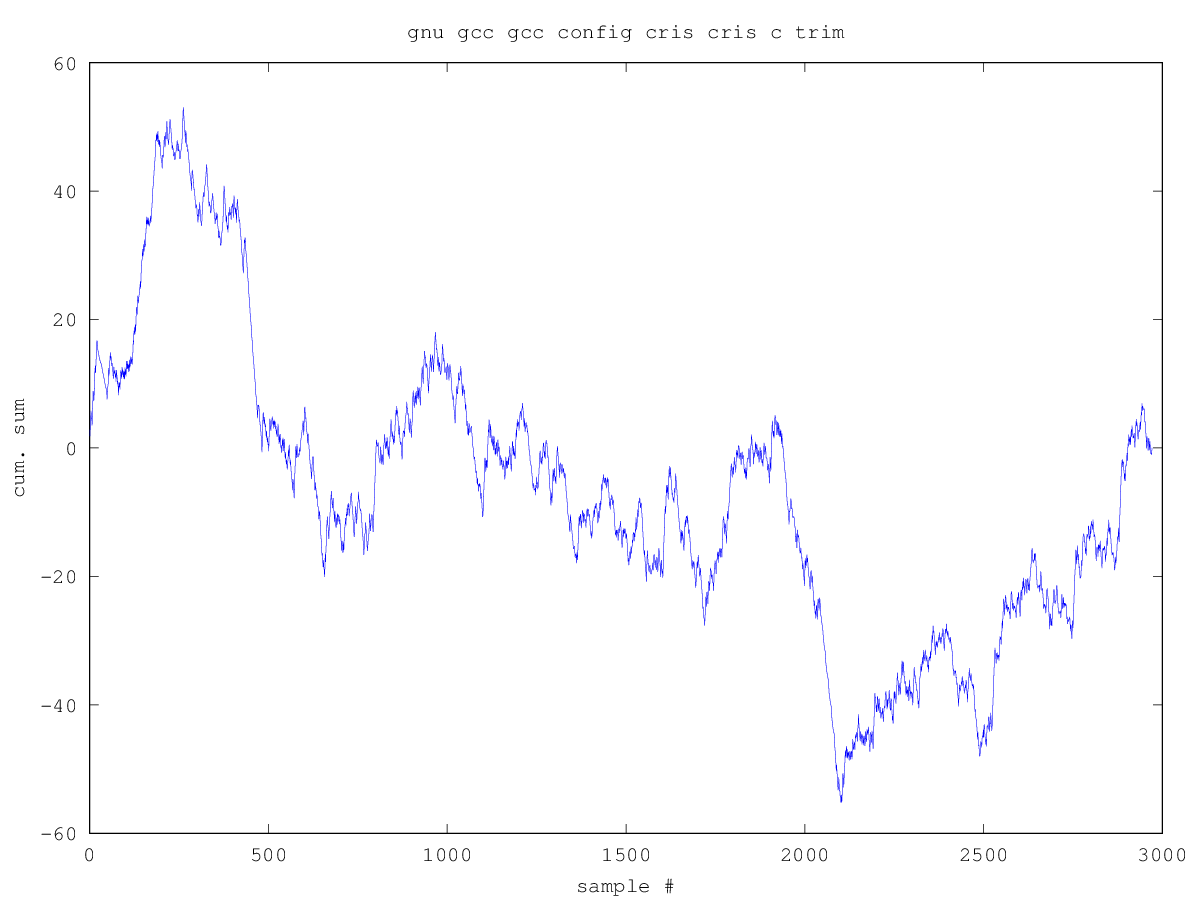
\includegraphics[width=0.8\linewidth]{{fractals/data/gnu_gcc_gcc_config_cris_cris_c_trim_time_series}.png}
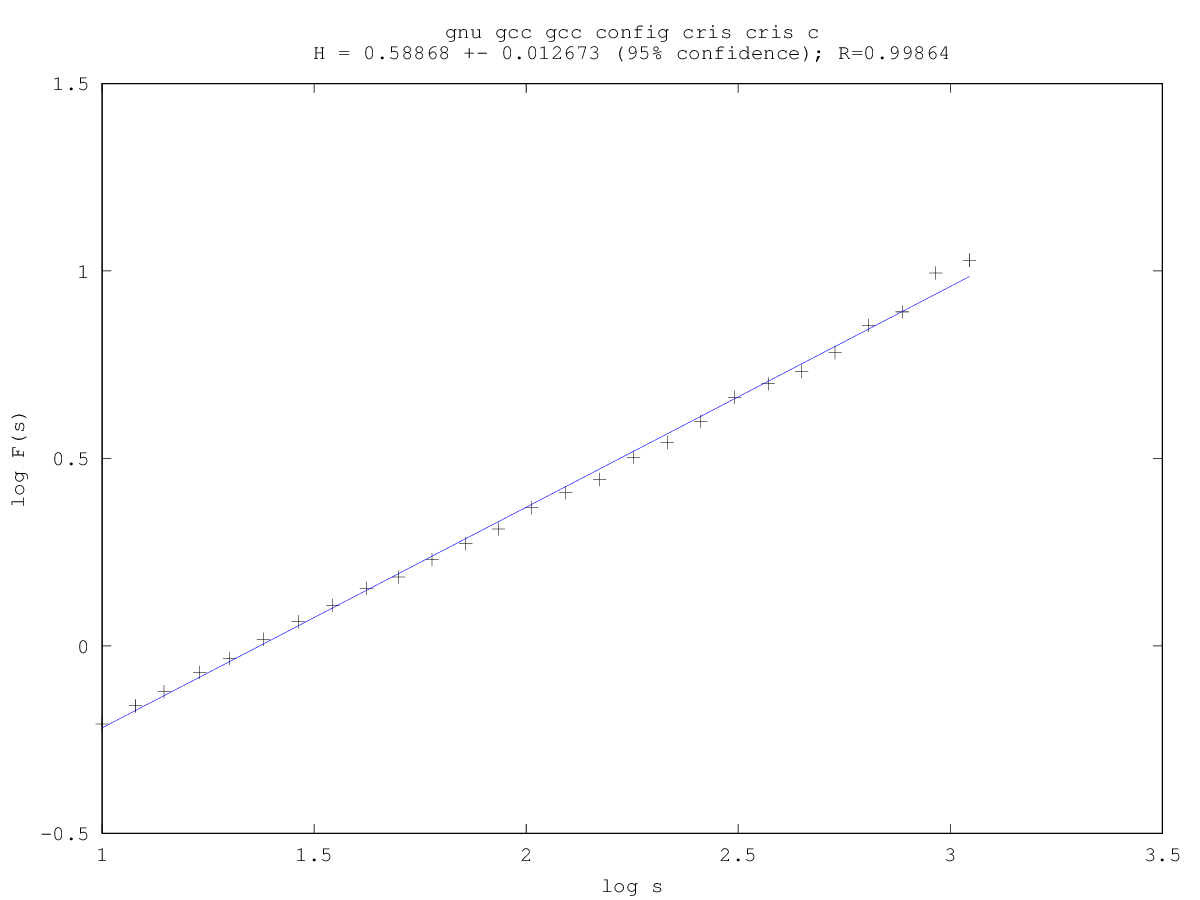
\includegraphics[width=0.8\linewidth]{{fractals/data/gnu_gcc_gcc_config_cris_cris_c_trim_log_log}.png}
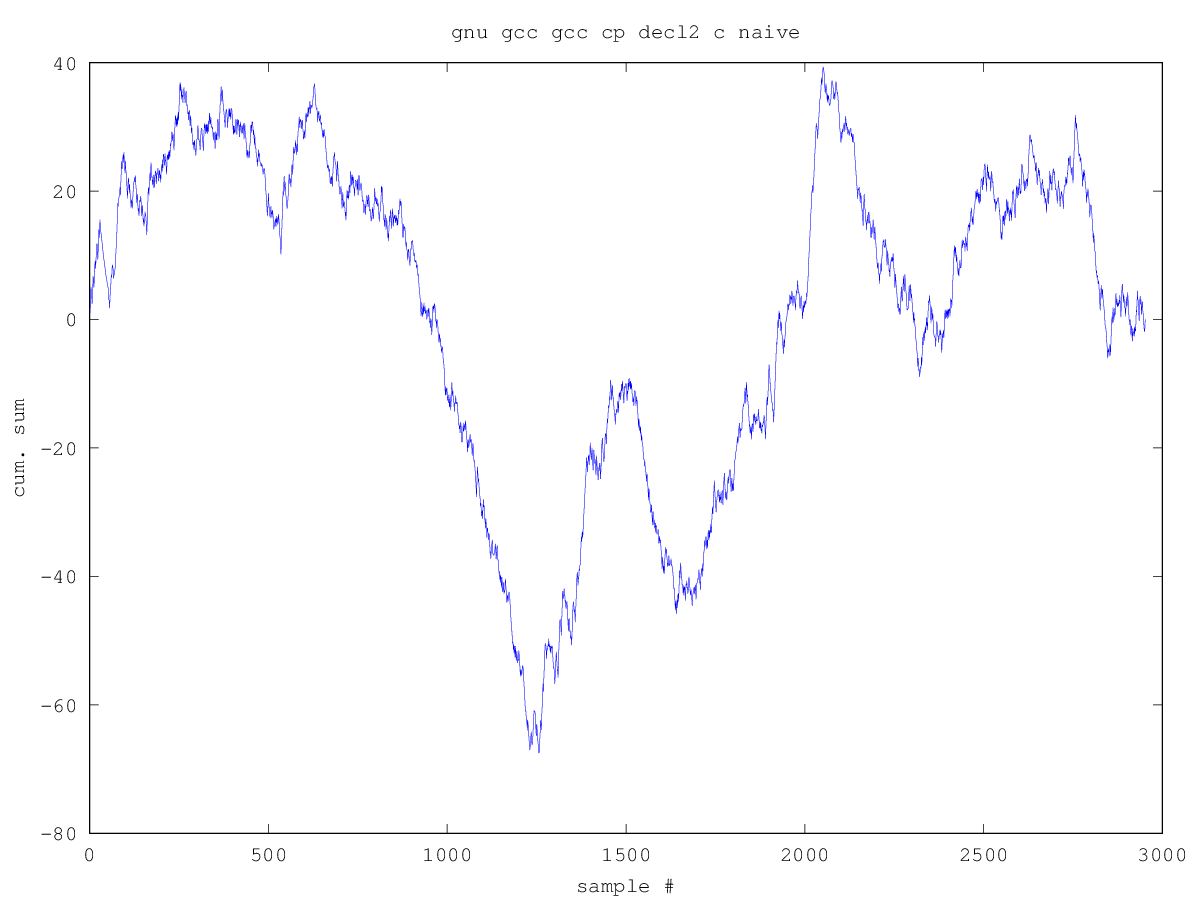
\includegraphics[width=0.8\linewidth]{{fractals/data/gnu_gcc_gcc_cp_decl2_c_naive_time_series}.png}
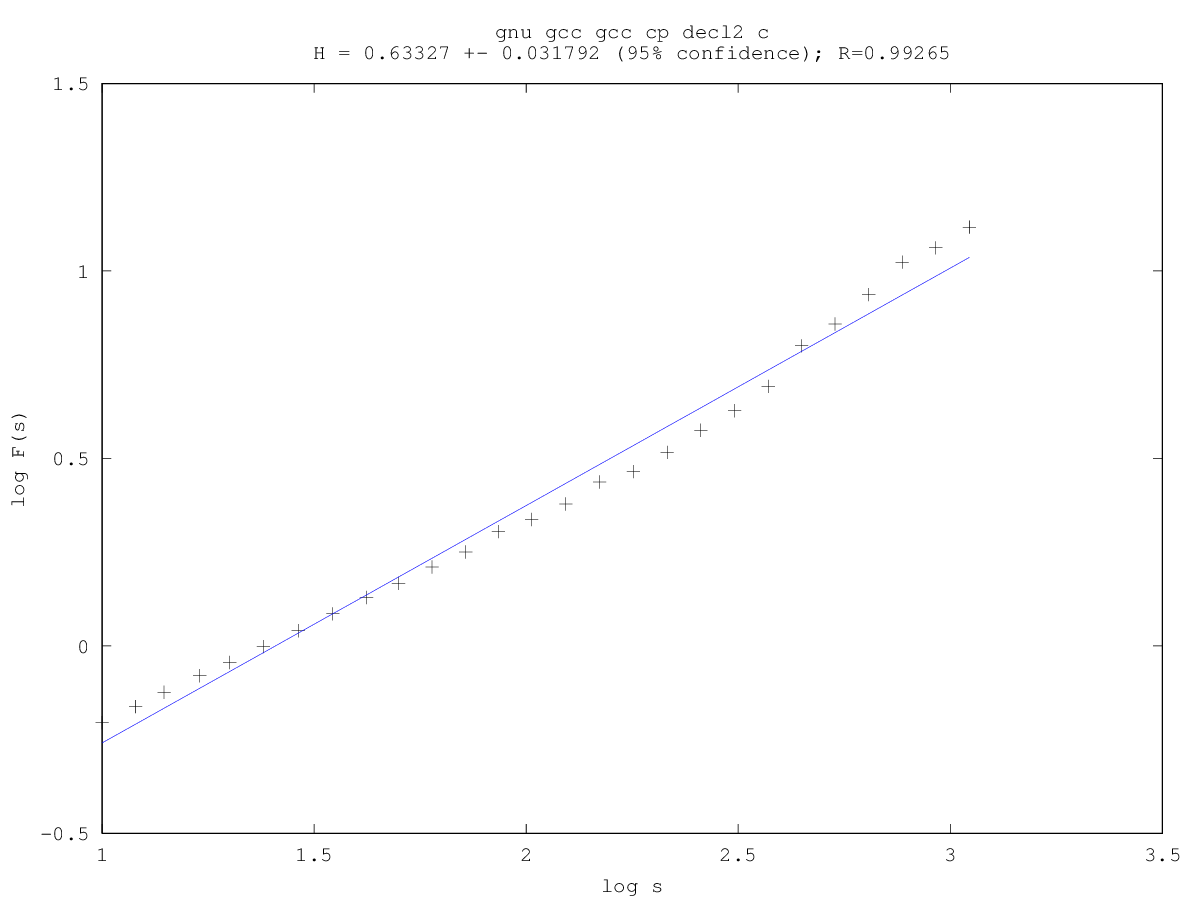
\includegraphics[width=0.8\linewidth]{{fractals/data/gnu_gcc_gcc_cp_decl2_c_naive_log_log}.png}
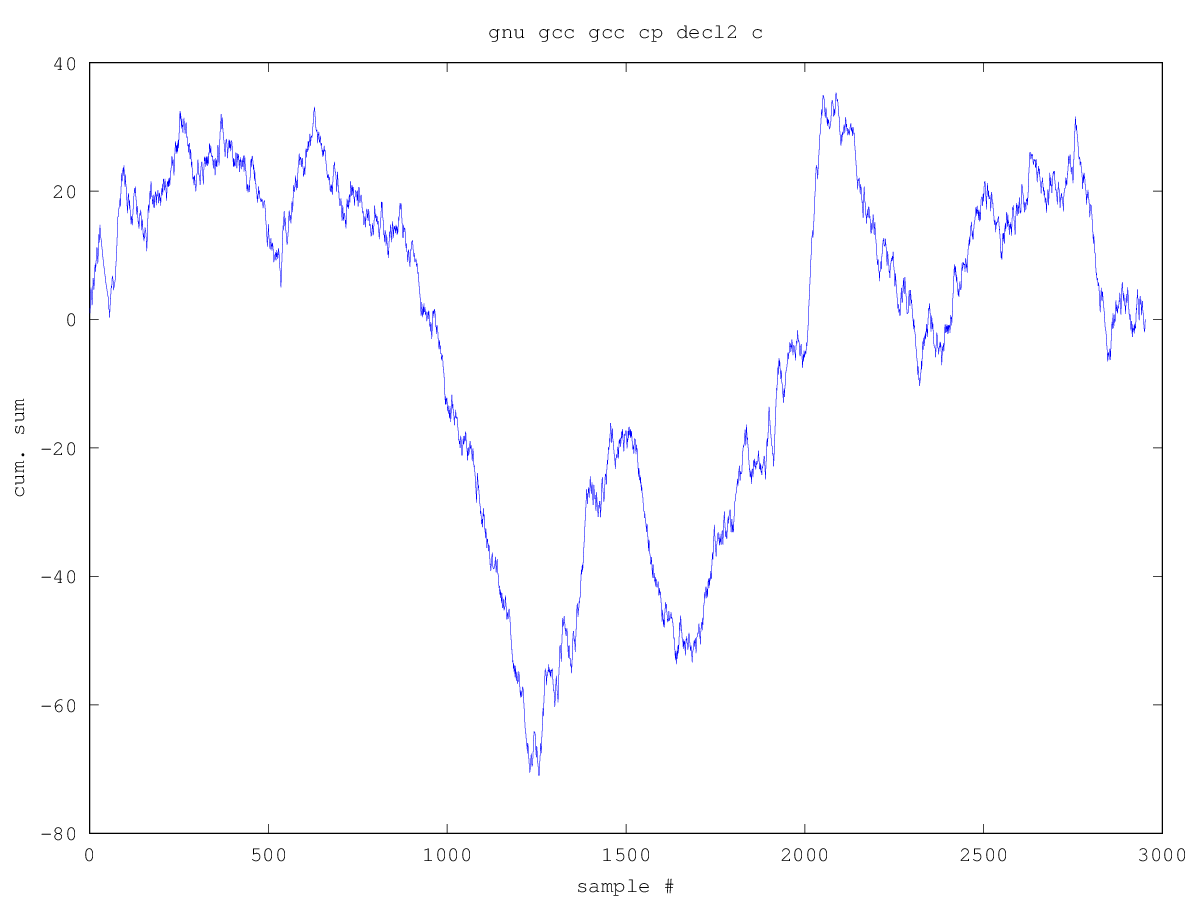
\includegraphics[width=0.8\linewidth]{{fractals/data/gnu_gcc_gcc_cp_decl2_c_tab3_time_series}.png}
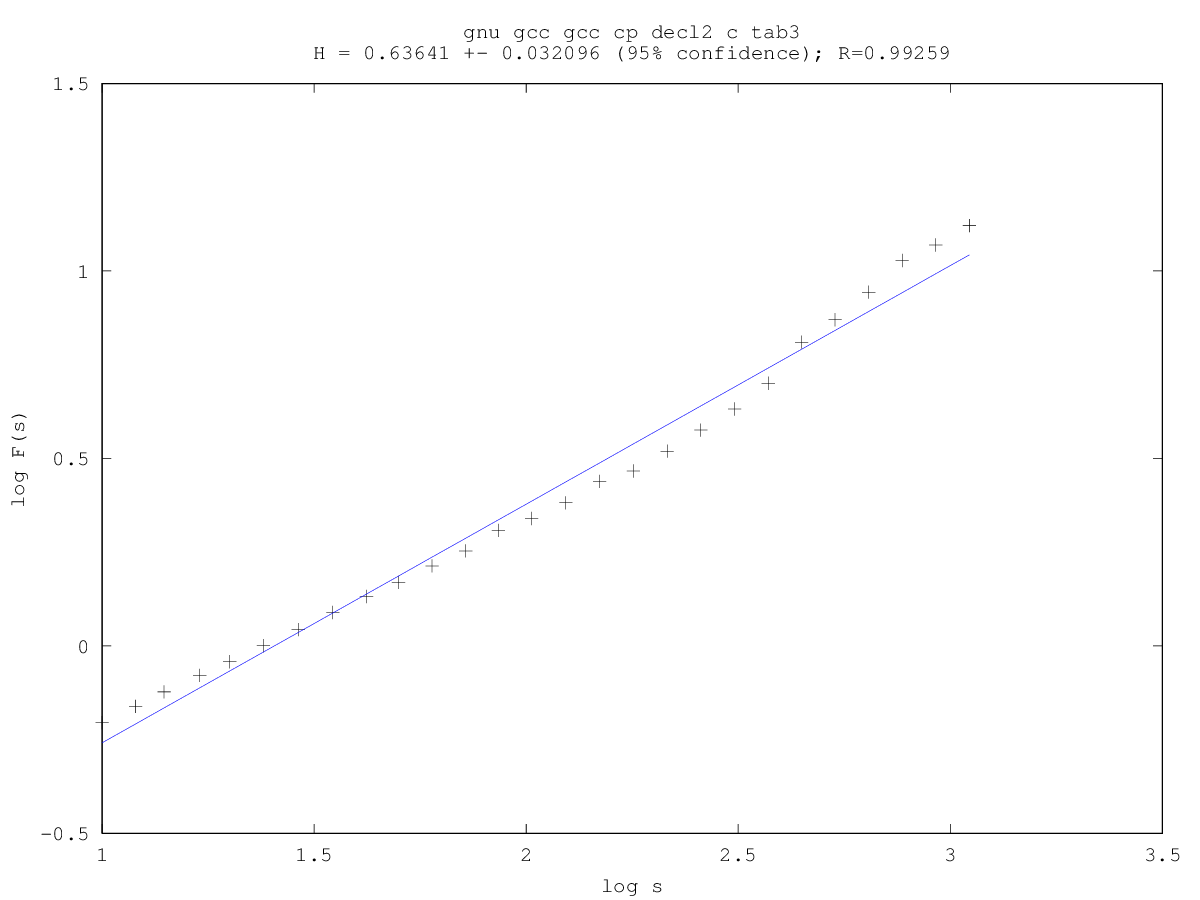
\includegraphics[width=0.8\linewidth]{{fractals/data/gnu_gcc_gcc_cp_decl2_c_tab3_log_log}.png}
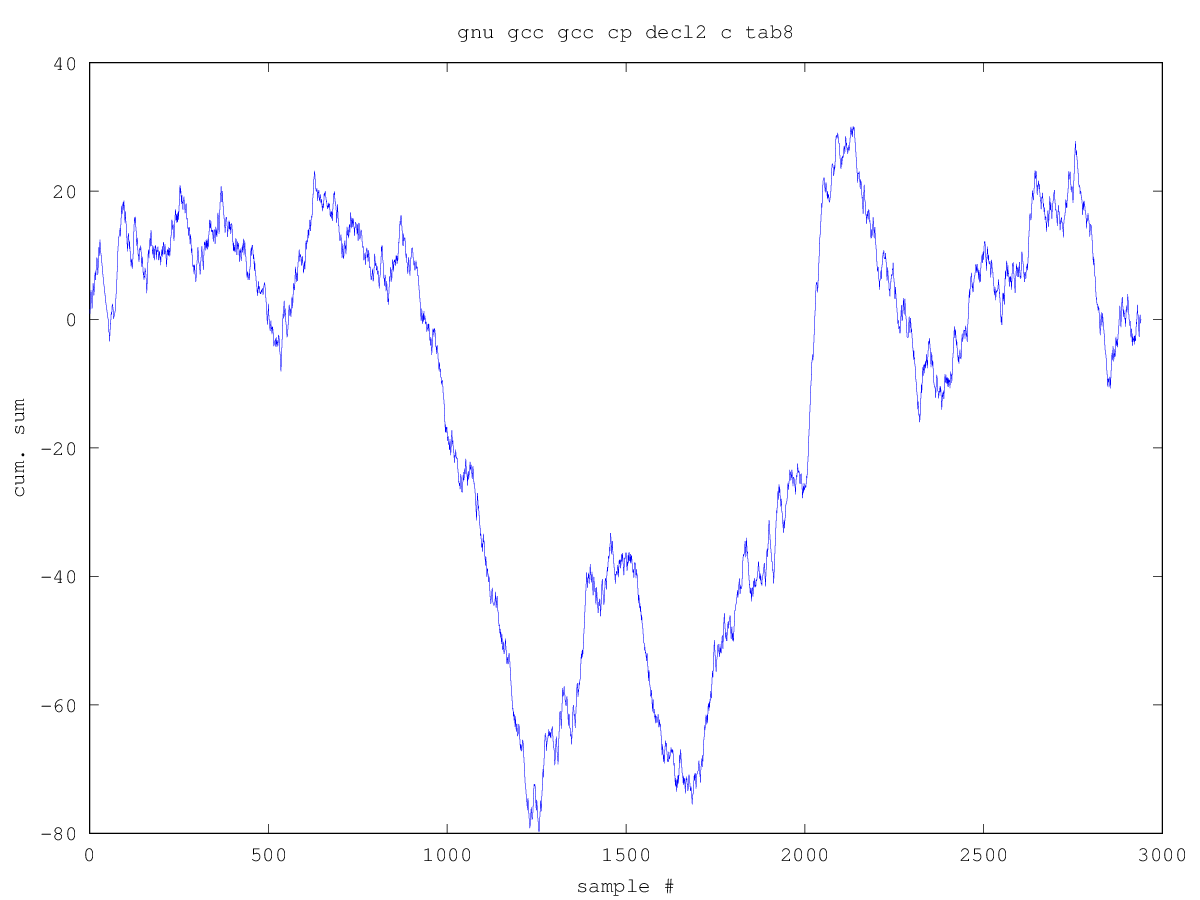
\includegraphics[width=0.8\linewidth]{{fractals/data/gnu_gcc_gcc_cp_decl2_c_tab8_time_series}.png}
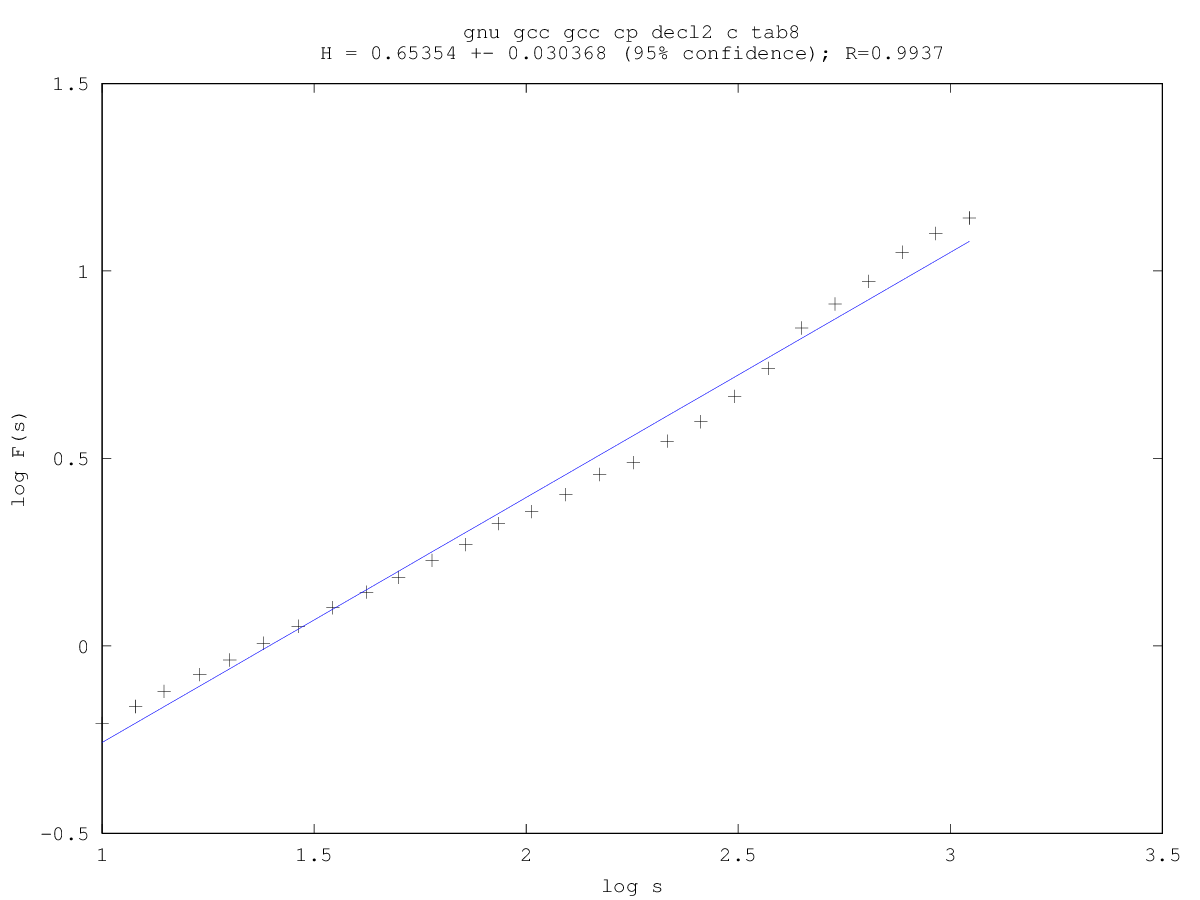
\includegraphics[width=0.8\linewidth]{{fractals/data/gnu_gcc_gcc_cp_decl2_c_tab8_log_log}.png}
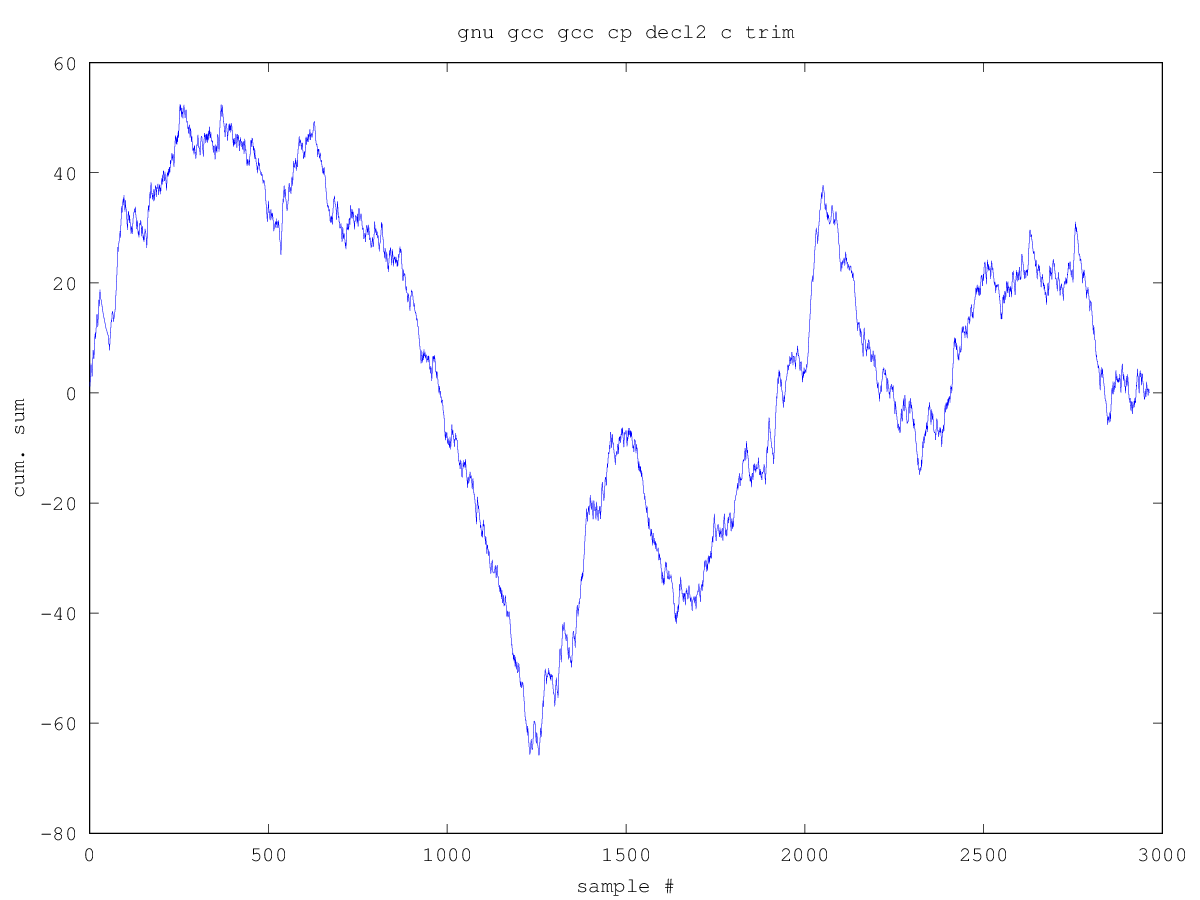
\includegraphics[width=0.8\linewidth]{{fractals/data/gnu_gcc_gcc_cp_decl2_c_trim_time_series}.png}
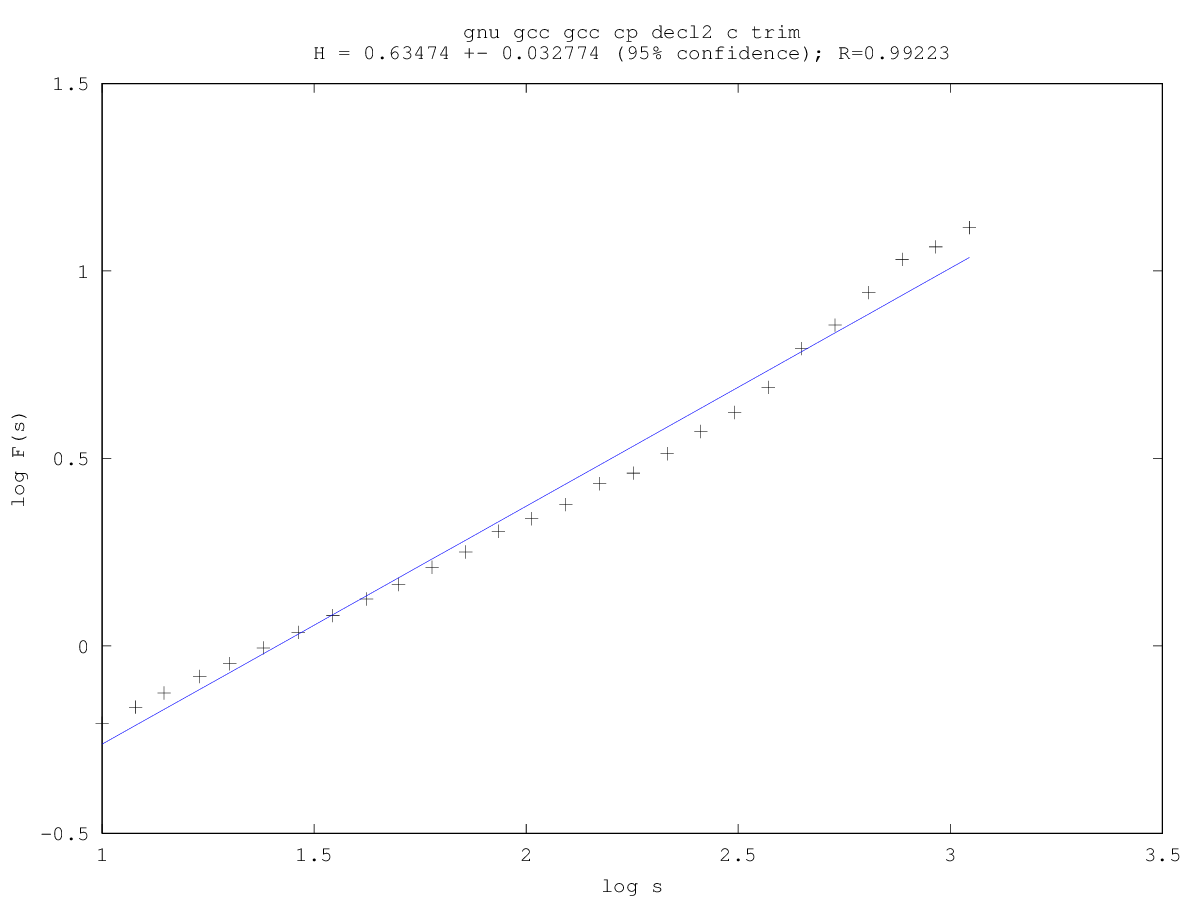
\includegraphics[width=0.8\linewidth]{{fractals/data/gnu_gcc_gcc_cp_decl2_c_trim_log_log}.png}
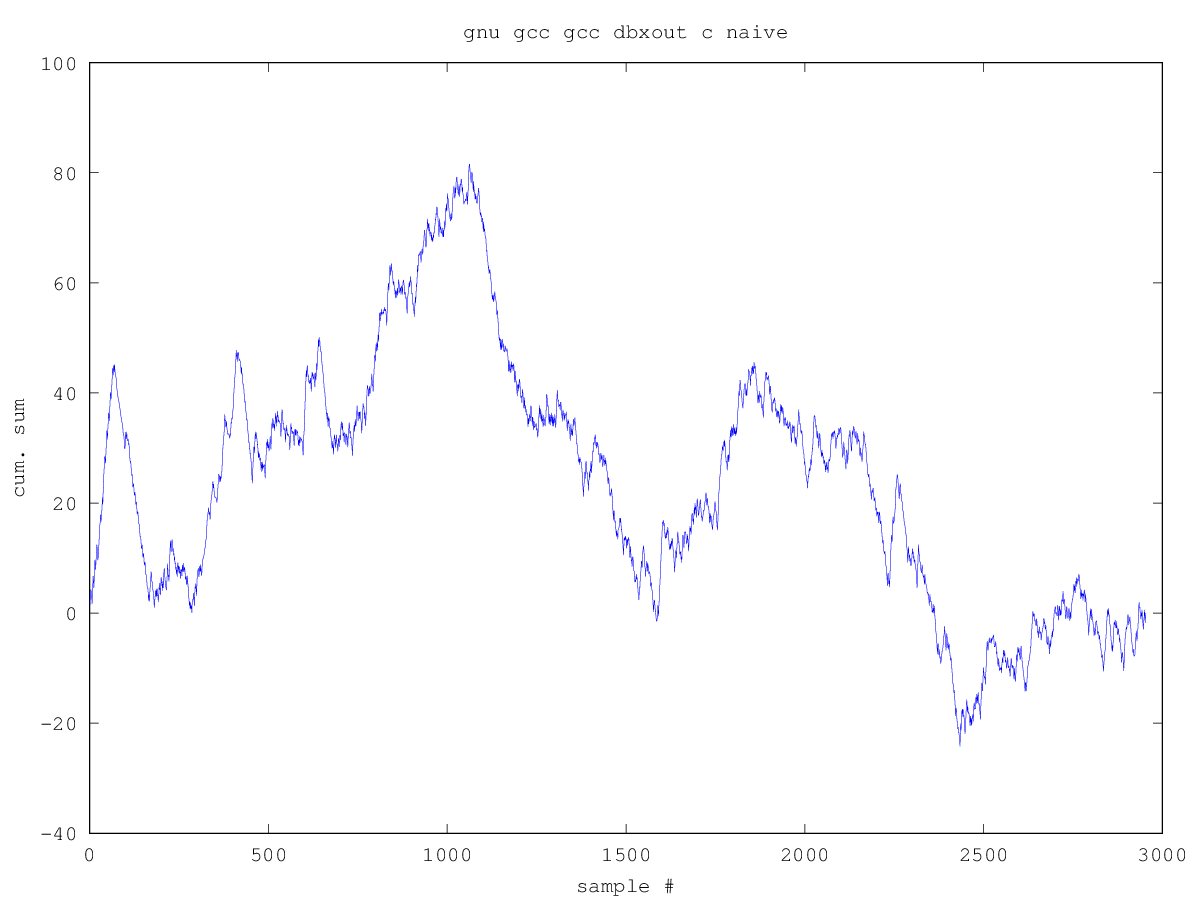
\includegraphics[width=0.8\linewidth]{{fractals/data/gnu_gcc_gcc_dbxout_c_naive_time_series}.png}
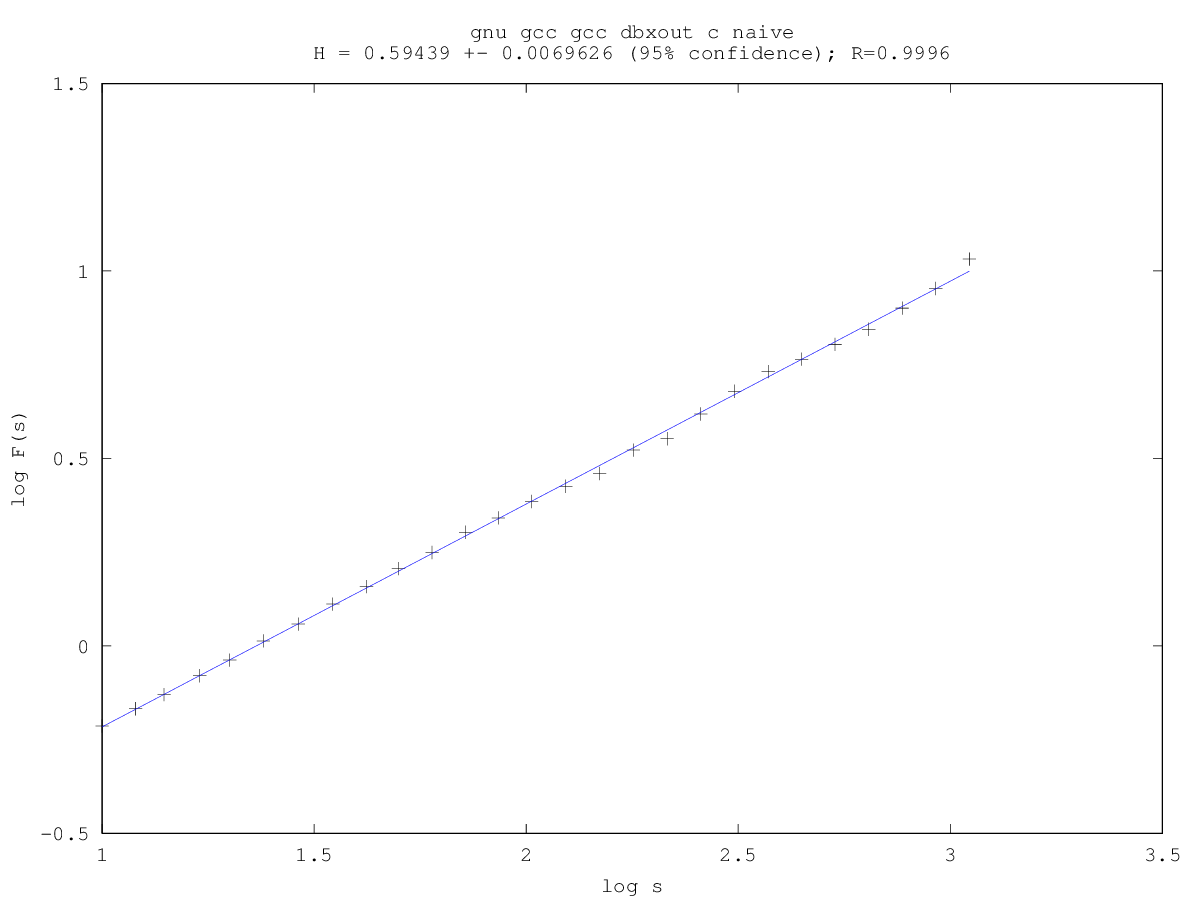
\includegraphics[width=0.8\linewidth]{{fractals/data/gnu_gcc_gcc_dbxout_c_naive_log_log}.png}
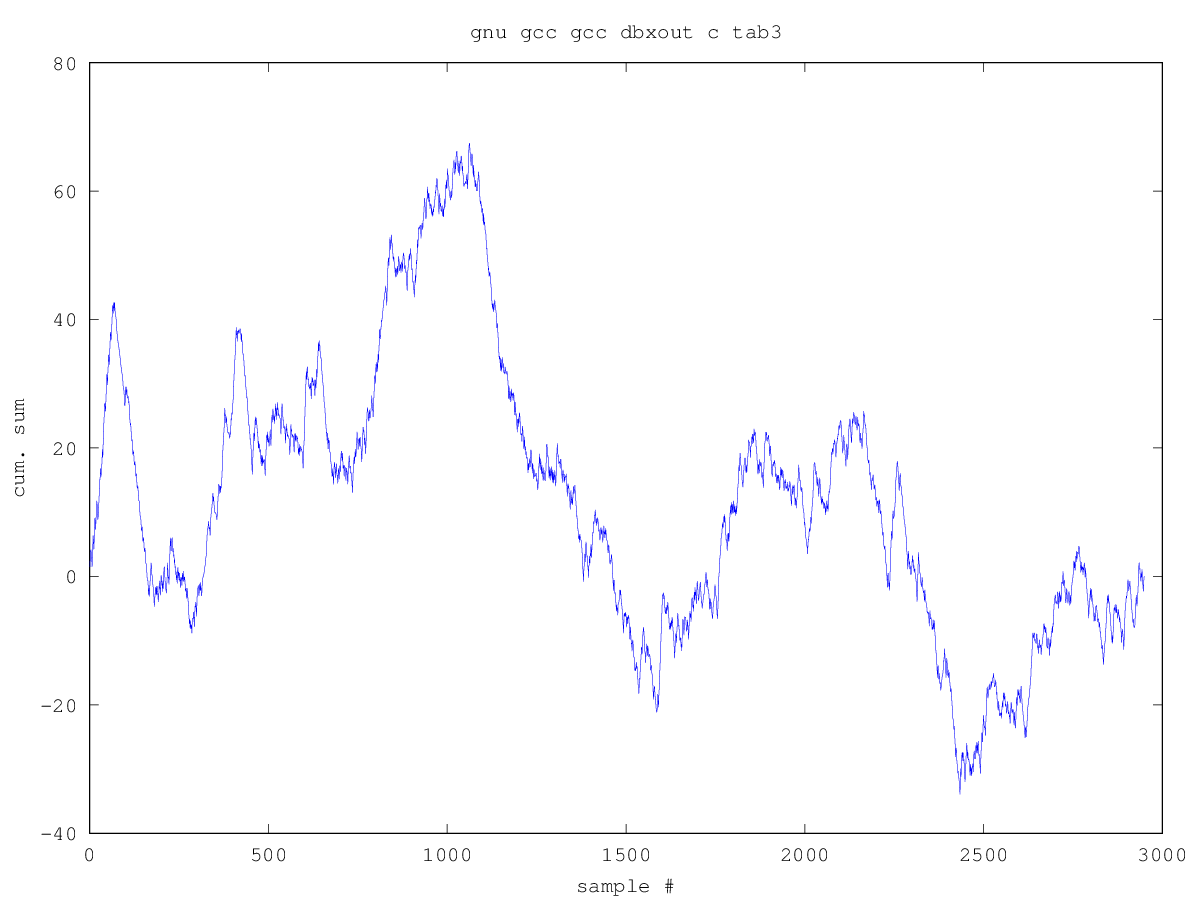
\includegraphics[width=0.8\linewidth]{{fractals/data/gnu_gcc_gcc_dbxout_c_tab3_time_series}.png}
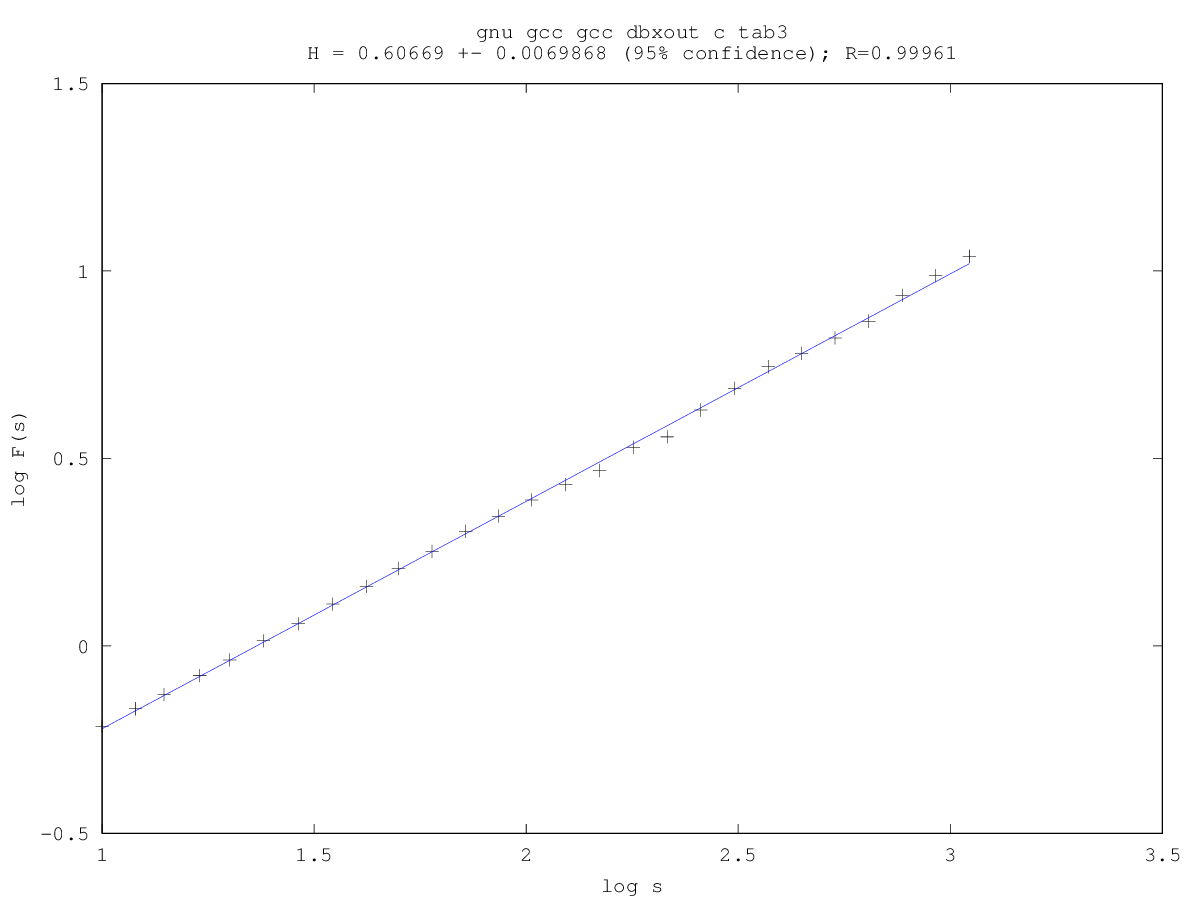
\includegraphics[width=0.8\linewidth]{{fractals/data/gnu_gcc_gcc_dbxout_c_tab3_log_log}.png}
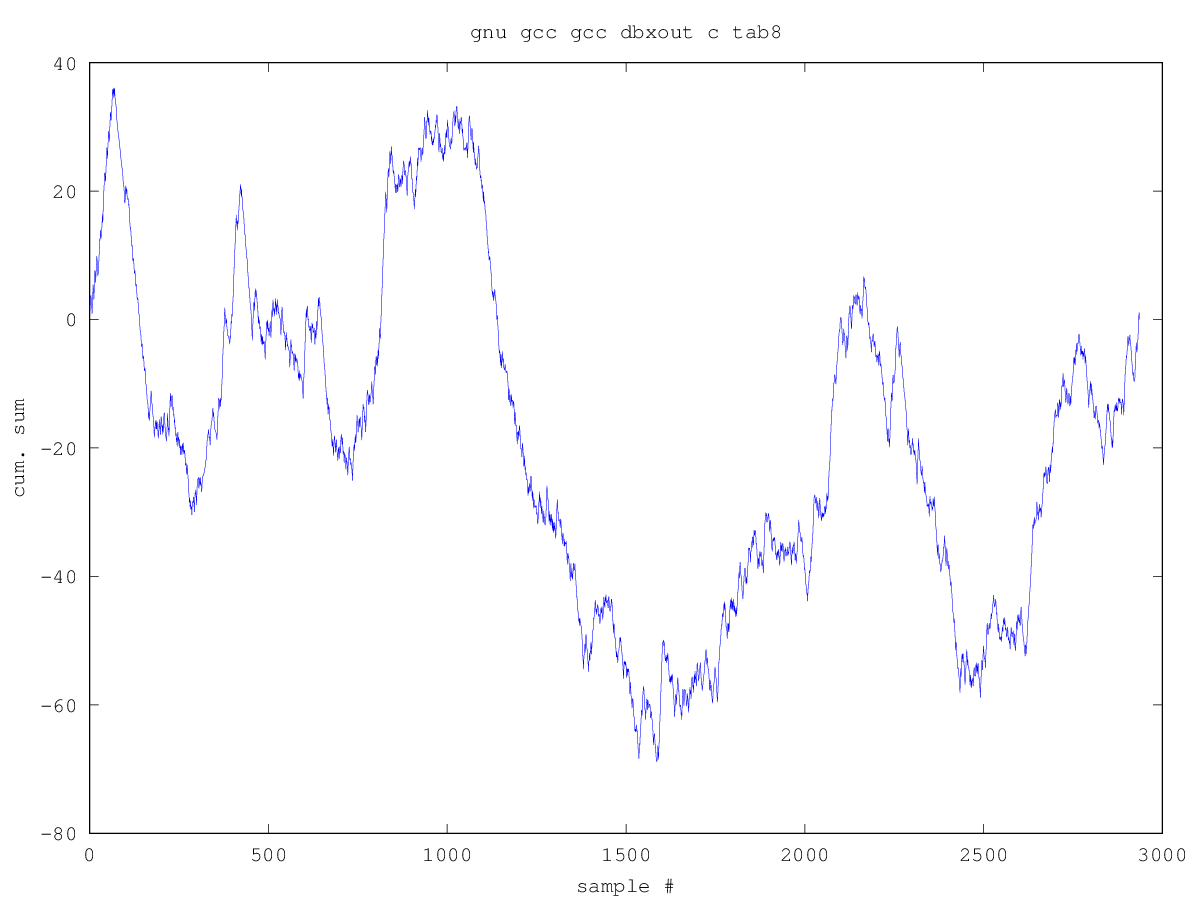
\includegraphics[width=0.8\linewidth]{{fractals/data/gnu_gcc_gcc_dbxout_c_tab8_time_series}.png}
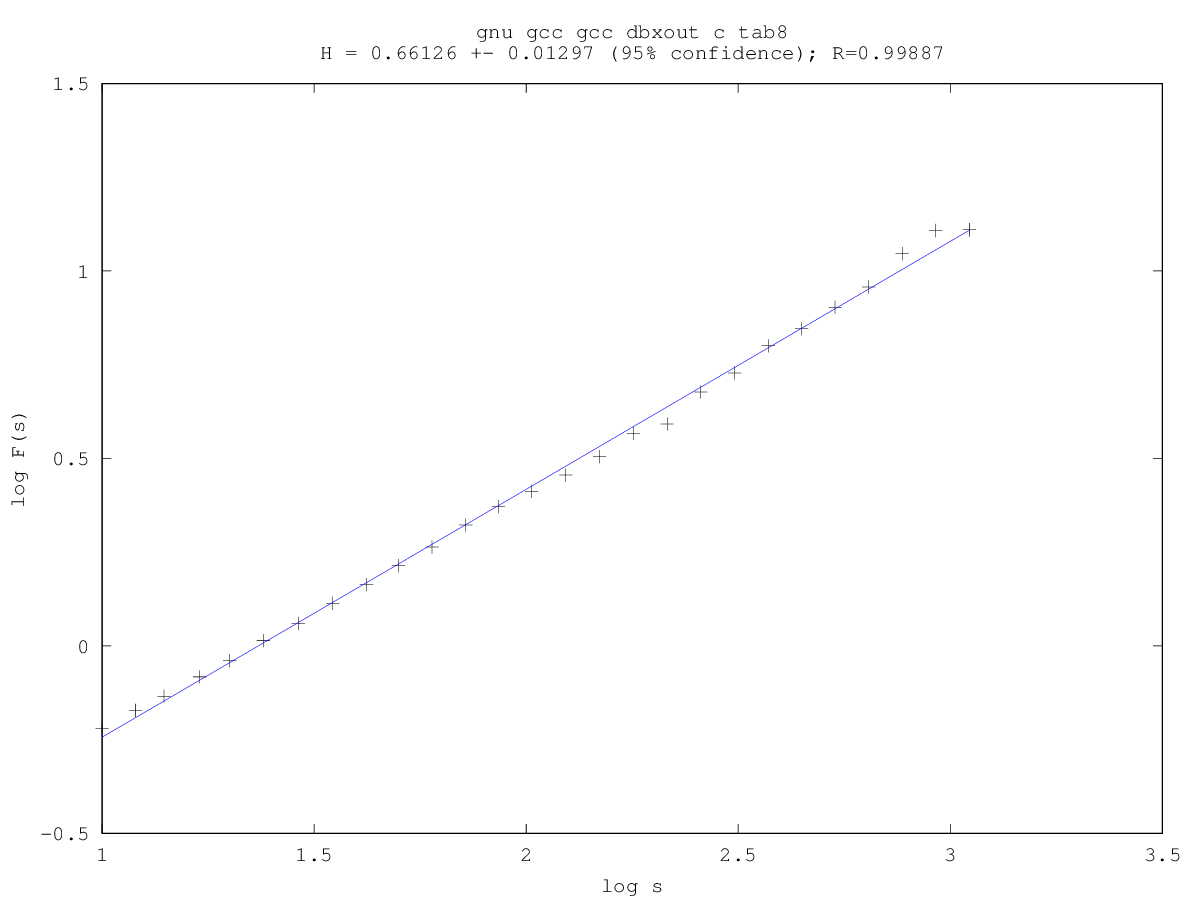
\includegraphics[width=0.8\linewidth]{{fractals/data/gnu_gcc_gcc_dbxout_c_tab8_log_log}.png}
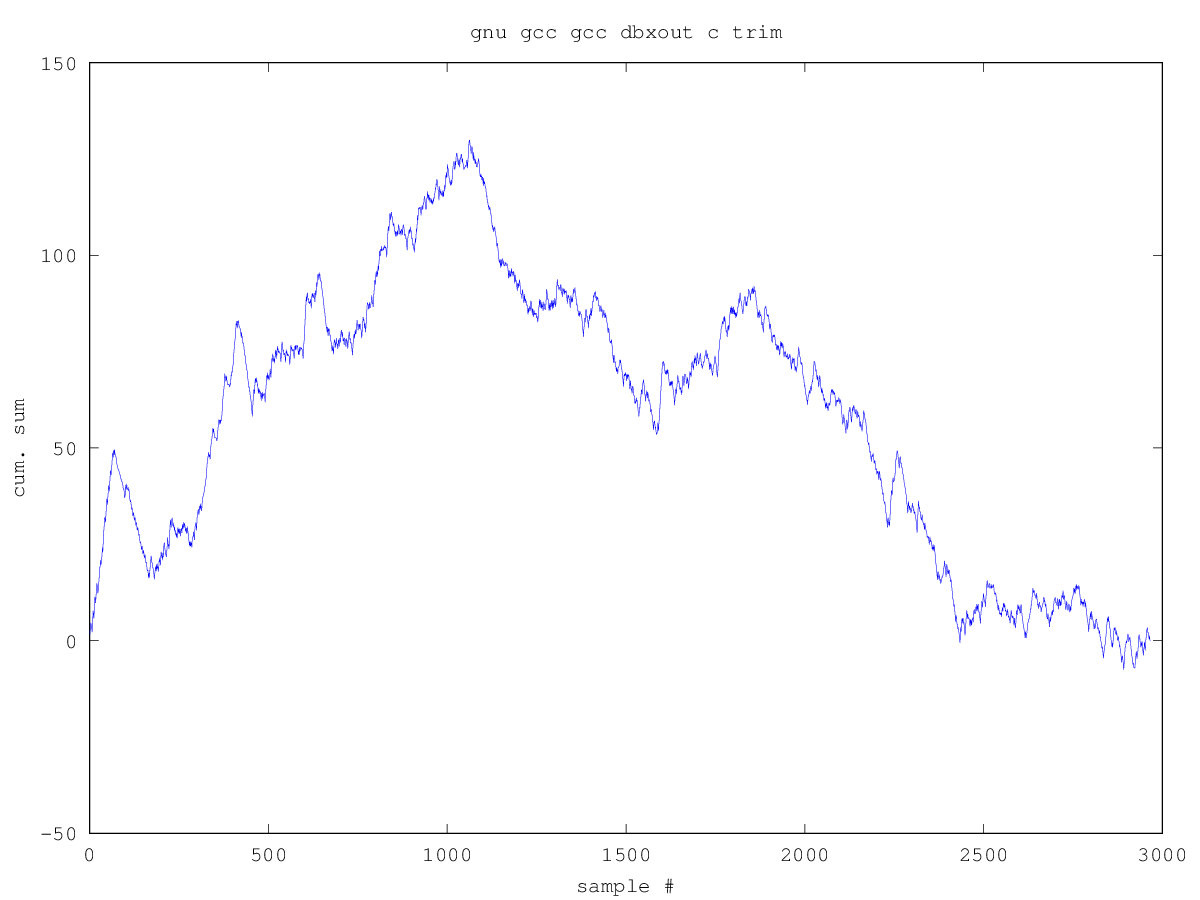
\includegraphics[width=0.8\linewidth]{{fractals/data/gnu_gcc_gcc_dbxout_c_trim_time_series}.png}
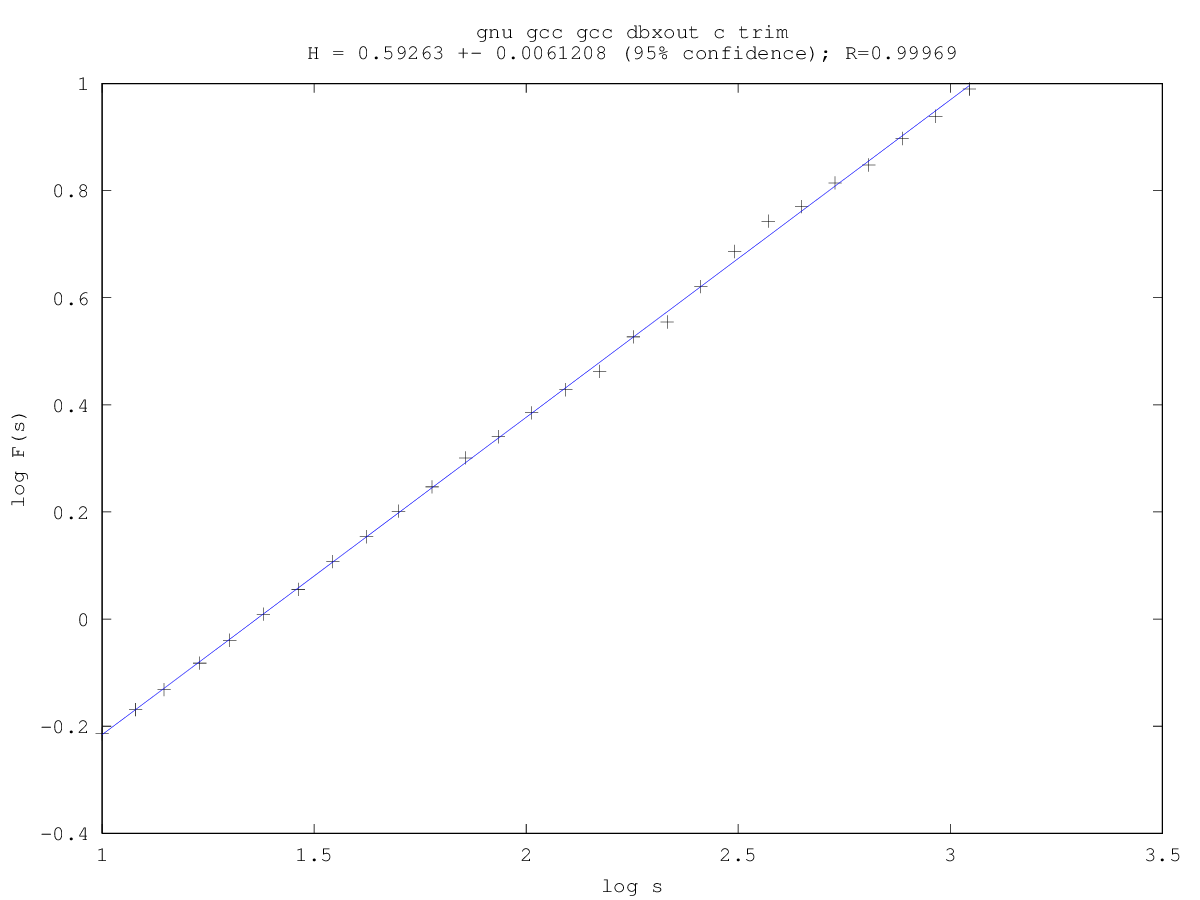
\includegraphics[width=0.8\linewidth]{{fractals/data/gnu_gcc_gcc_dbxout_c_trim_log_log}.png}
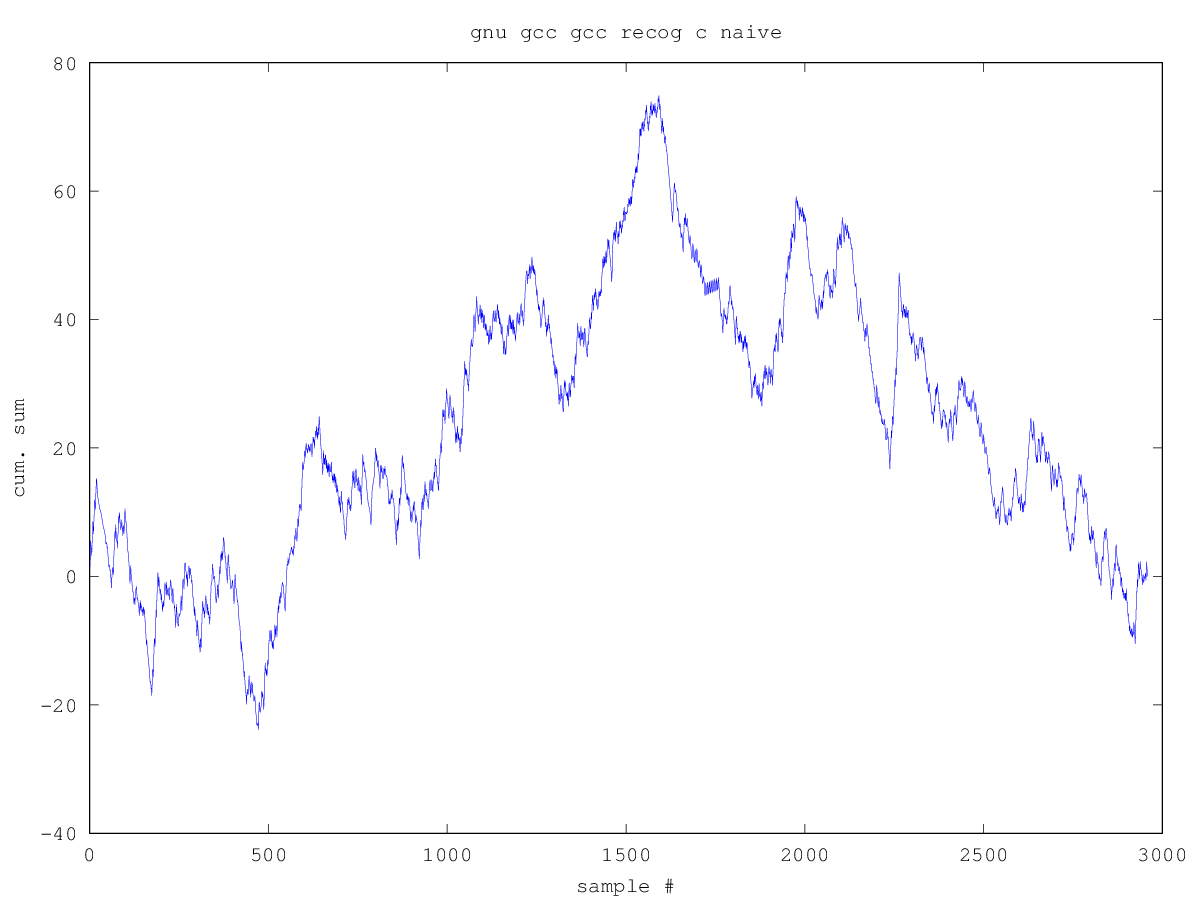
\includegraphics[width=0.8\linewidth]{{fractals/data/gnu_gcc_gcc_recog_c_naive_time_series}.png}
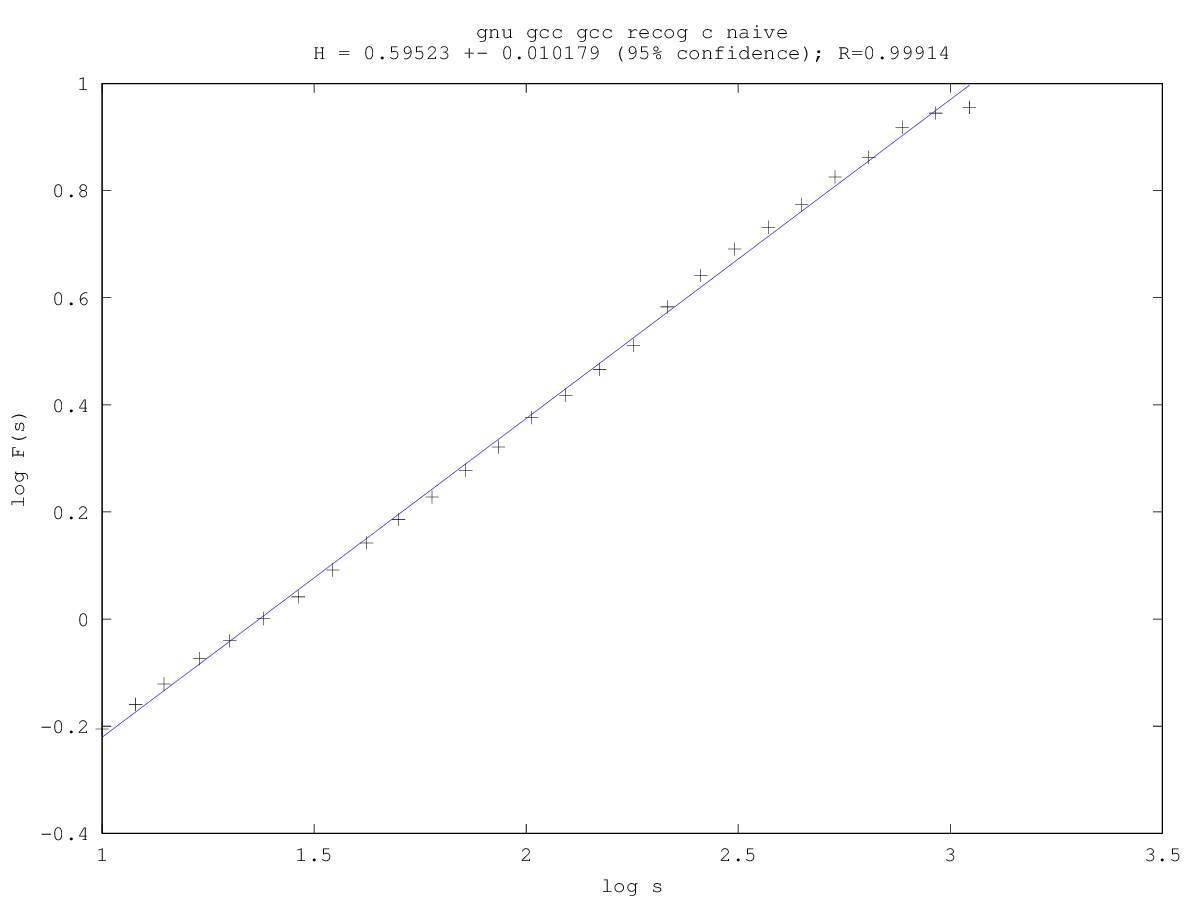
\includegraphics[width=0.8\linewidth]{{fractals/data/gnu_gcc_gcc_recog_c_naive_log_log}.png}
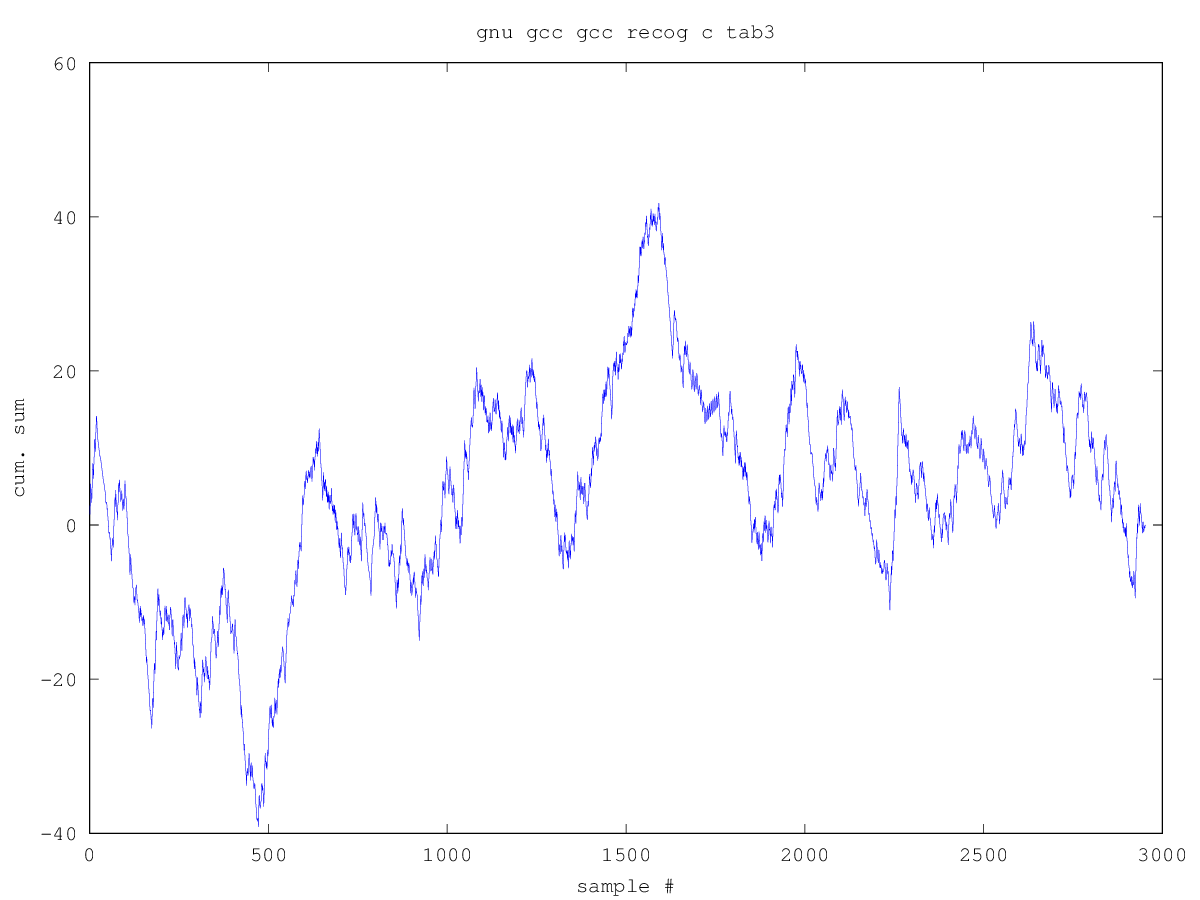
\includegraphics[width=0.8\linewidth]{{fractals/data/gnu_gcc_gcc_recog_c_tab3_time_series}.png}
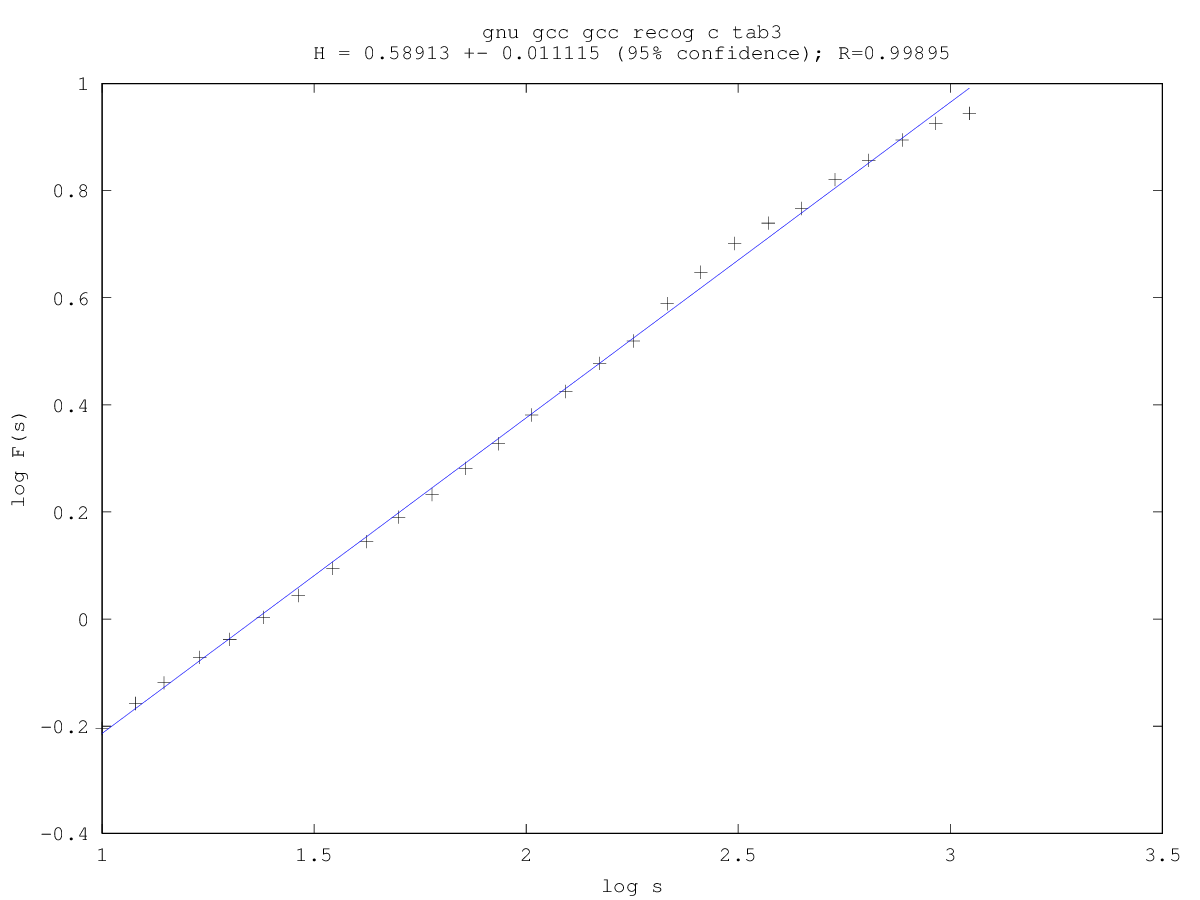
\includegraphics[width=0.8\linewidth]{{fractals/data/gnu_gcc_gcc_recog_c_tab3_log_log}.png}
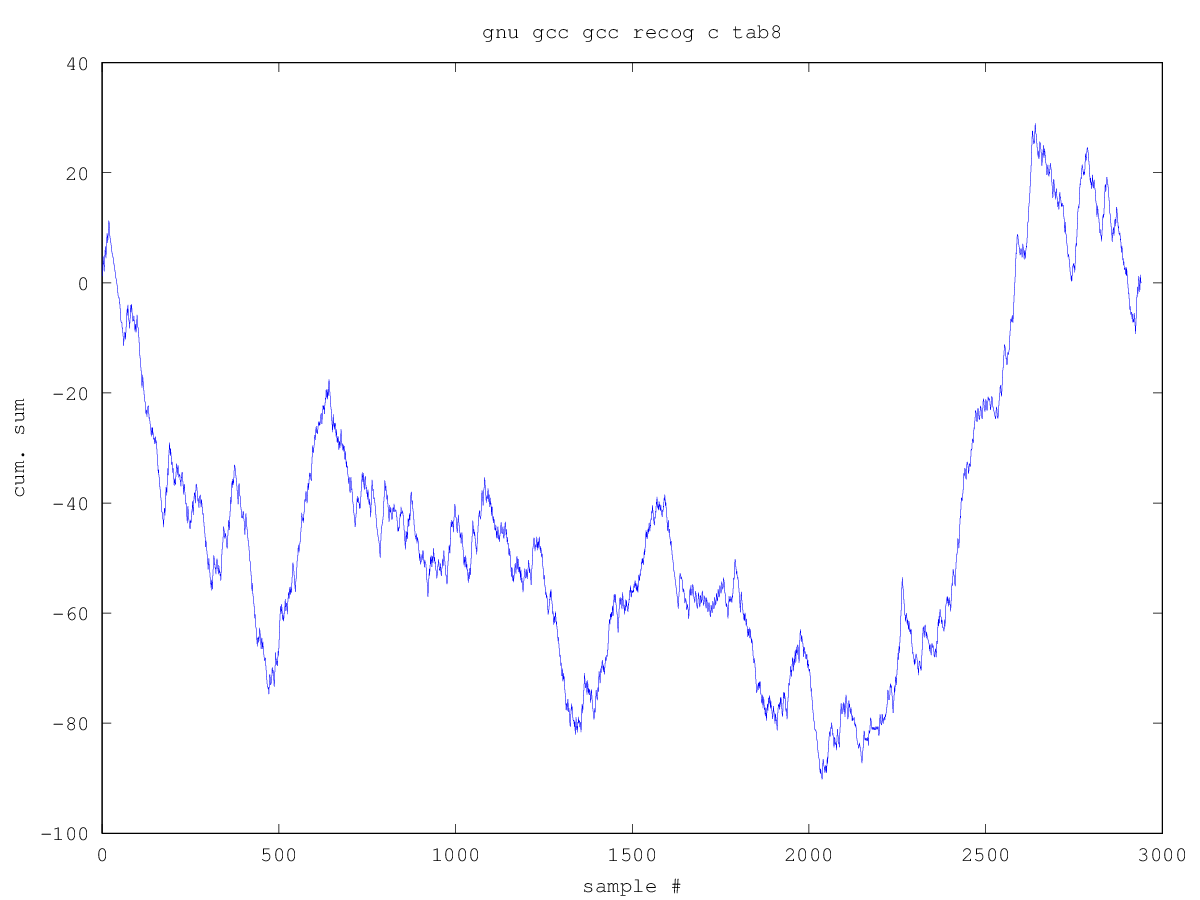
\includegraphics[width=0.8\linewidth]{{fractals/data/gnu_gcc_gcc_recog_c_tab8_time_series}.png}
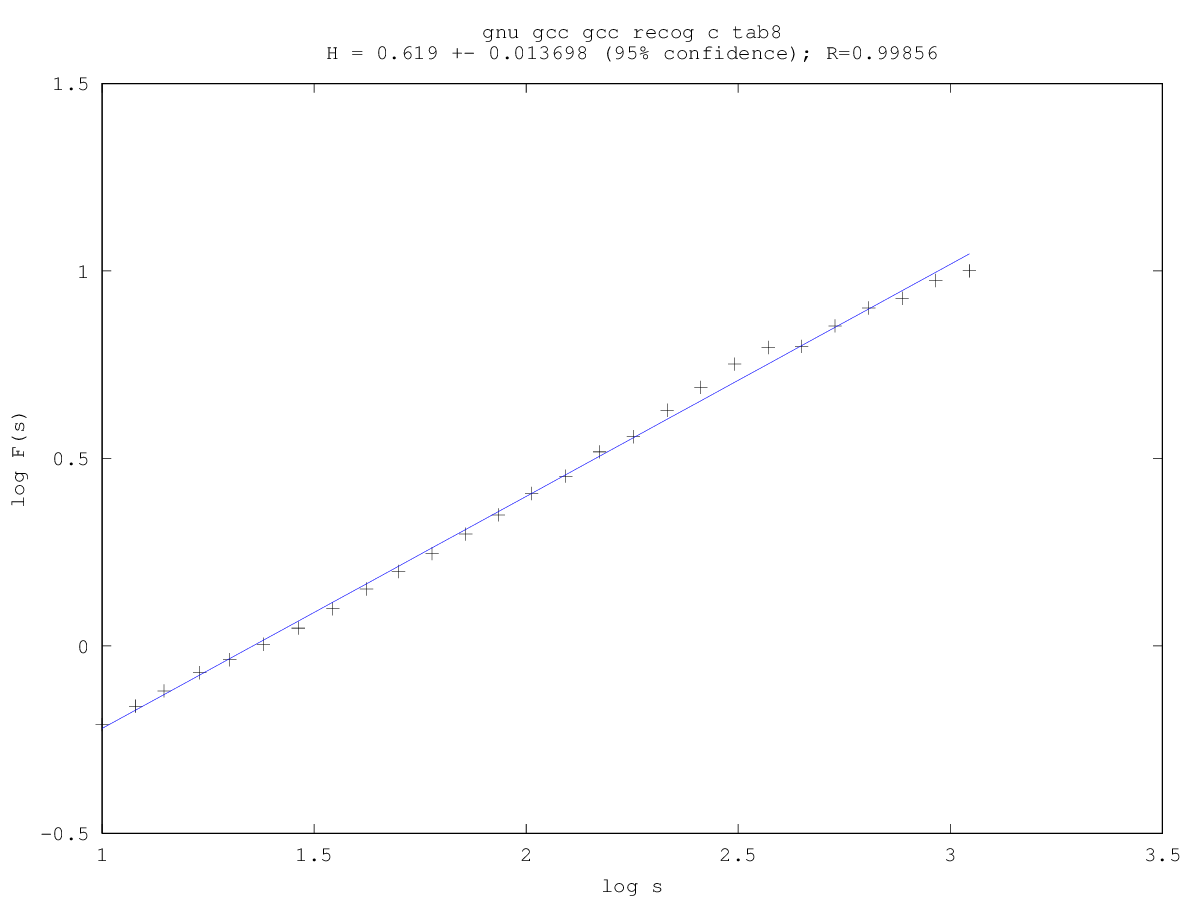
\includegraphics[width=0.8\linewidth]{{fractals/data/gnu_gcc_gcc_recog_c_tab8_log_log}.png}
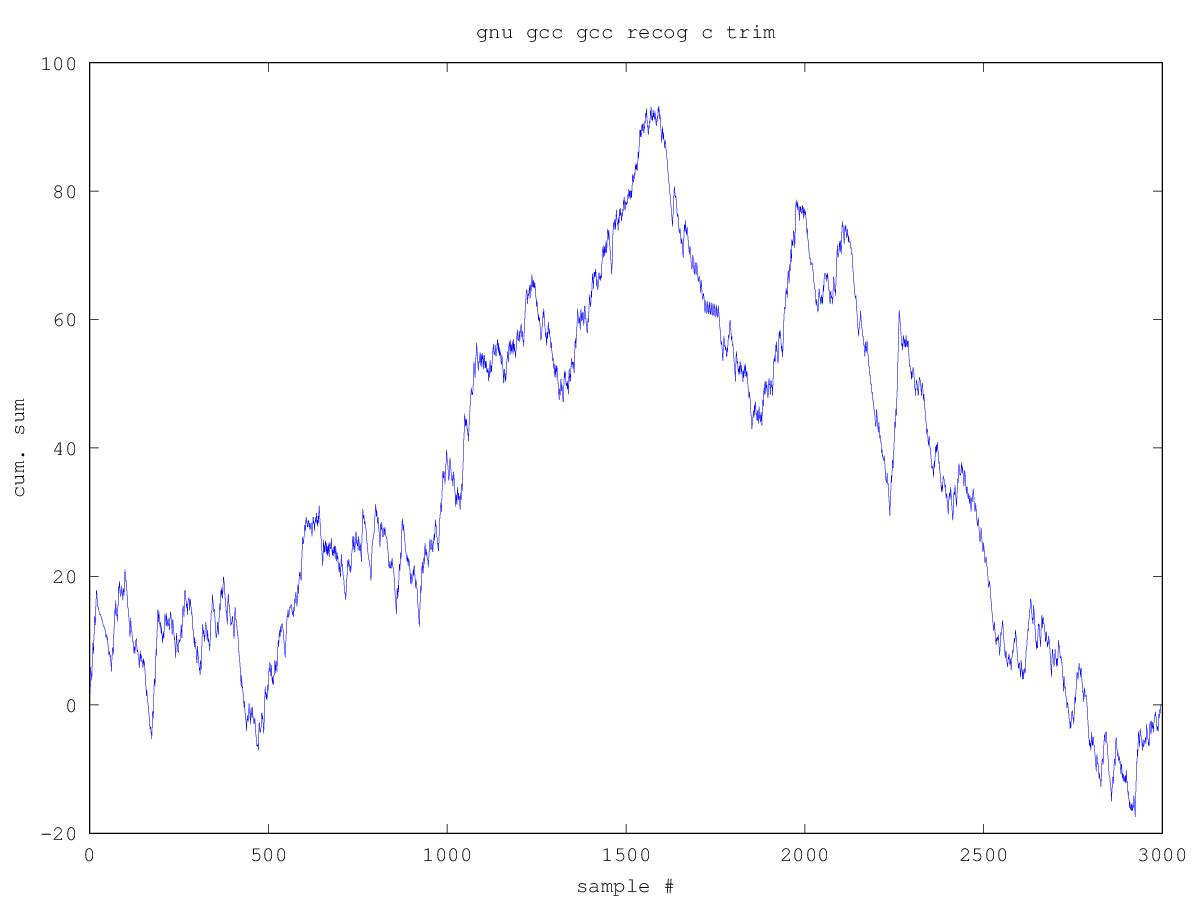
\includegraphics[width=0.8\linewidth]{{fractals/data/gnu_gcc_gcc_recog_c_trim_time_series}.png}
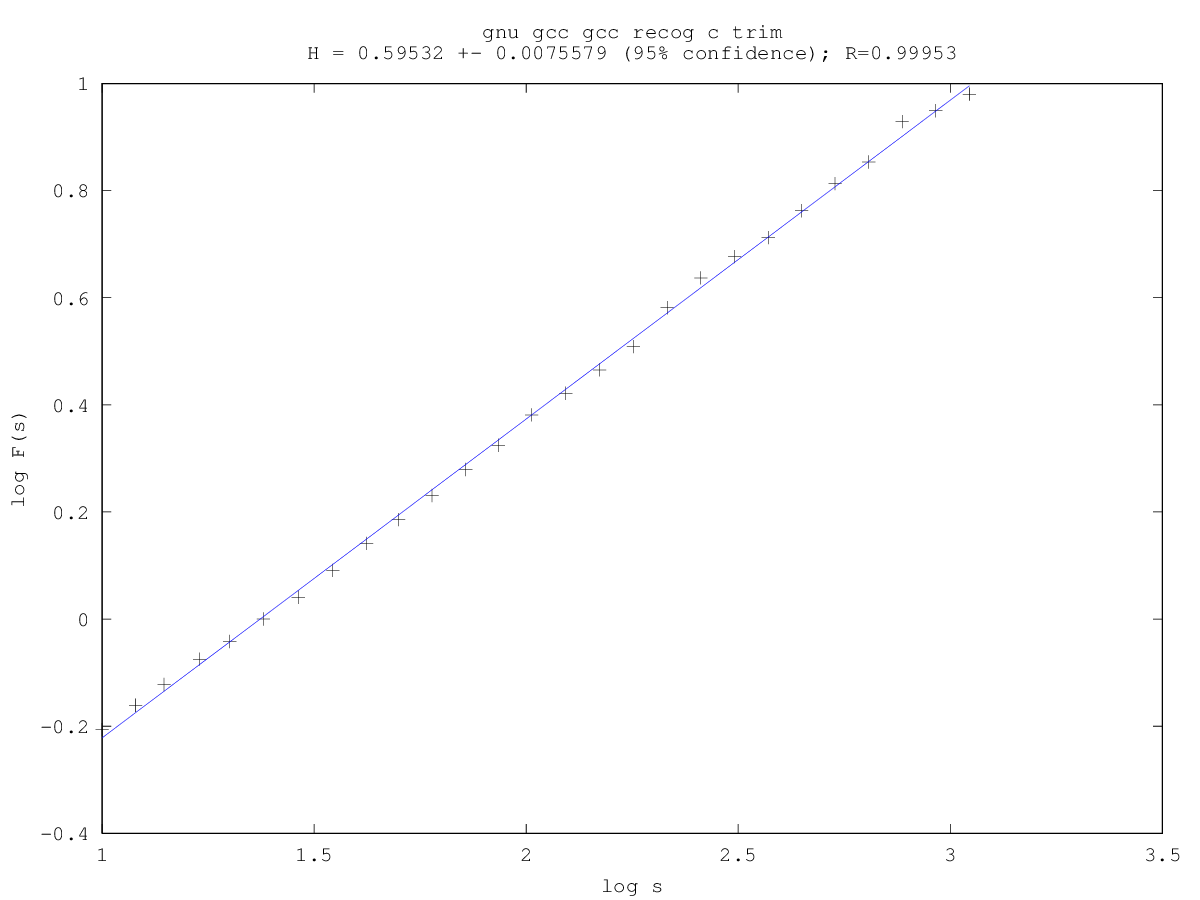
\includegraphics[width=0.8\linewidth]{{fractals/data/gnu_gcc_gcc_recog_c_trim_log_log}.png}
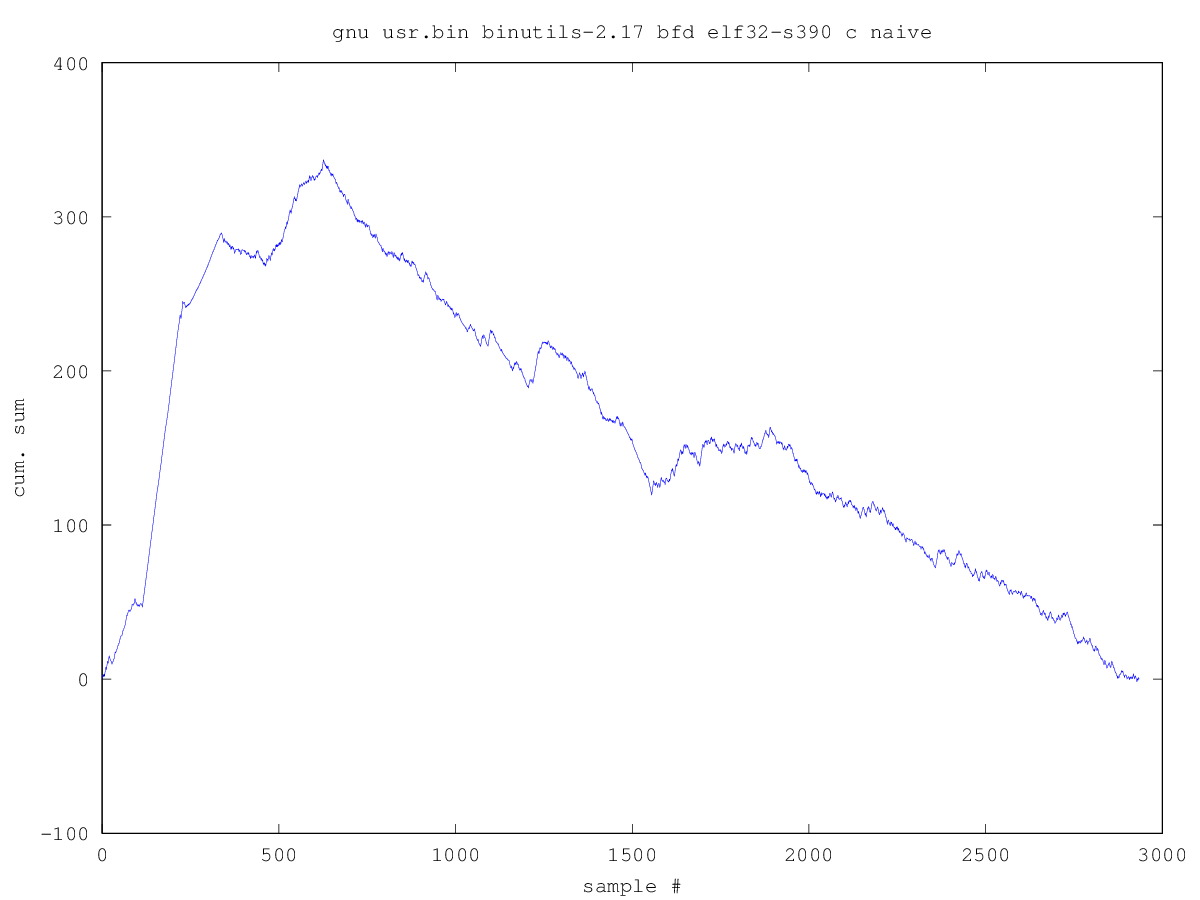
\includegraphics[width=0.8\linewidth]{{fractals/data/gnu_usr.bin_binutils-2.17_bfd_elf32-s390_c_naive_time_series}.png}
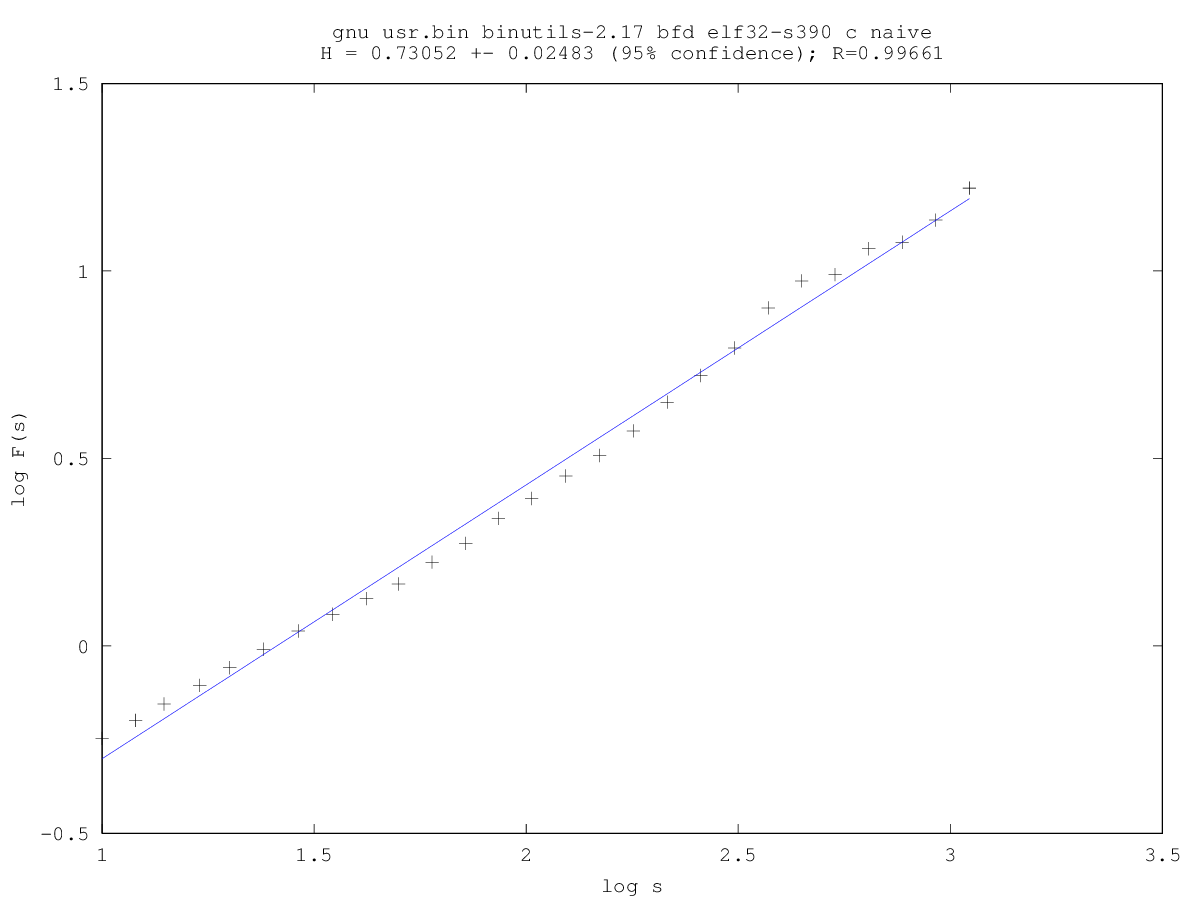
\includegraphics[width=0.8\linewidth]{{fractals/data/gnu_usr.bin_binutils-2.17_bfd_elf32-s390_c_naive_log_log}.png}
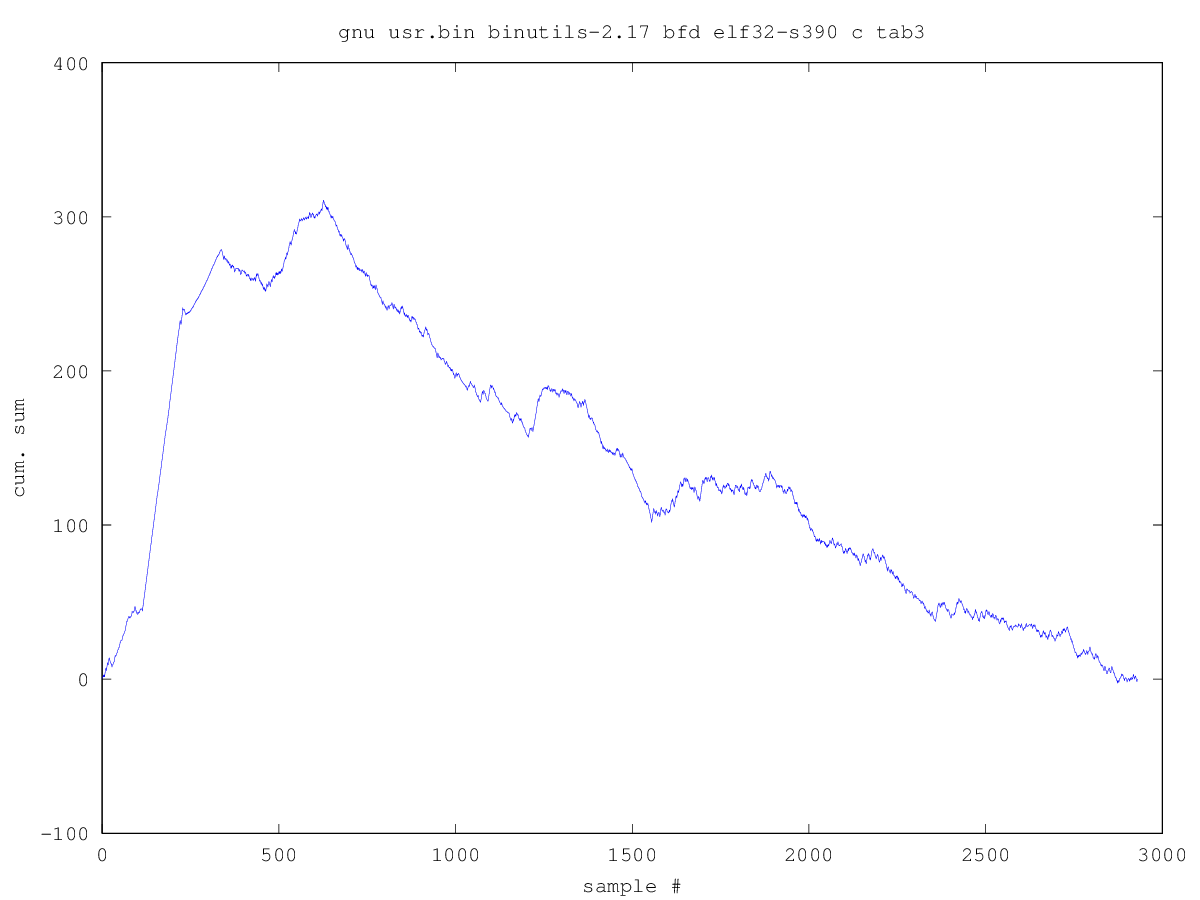
\includegraphics[width=0.8\linewidth]{{fractals/data/gnu_usr.bin_binutils-2.17_bfd_elf32-s390_c_tab3_time_series}.png}
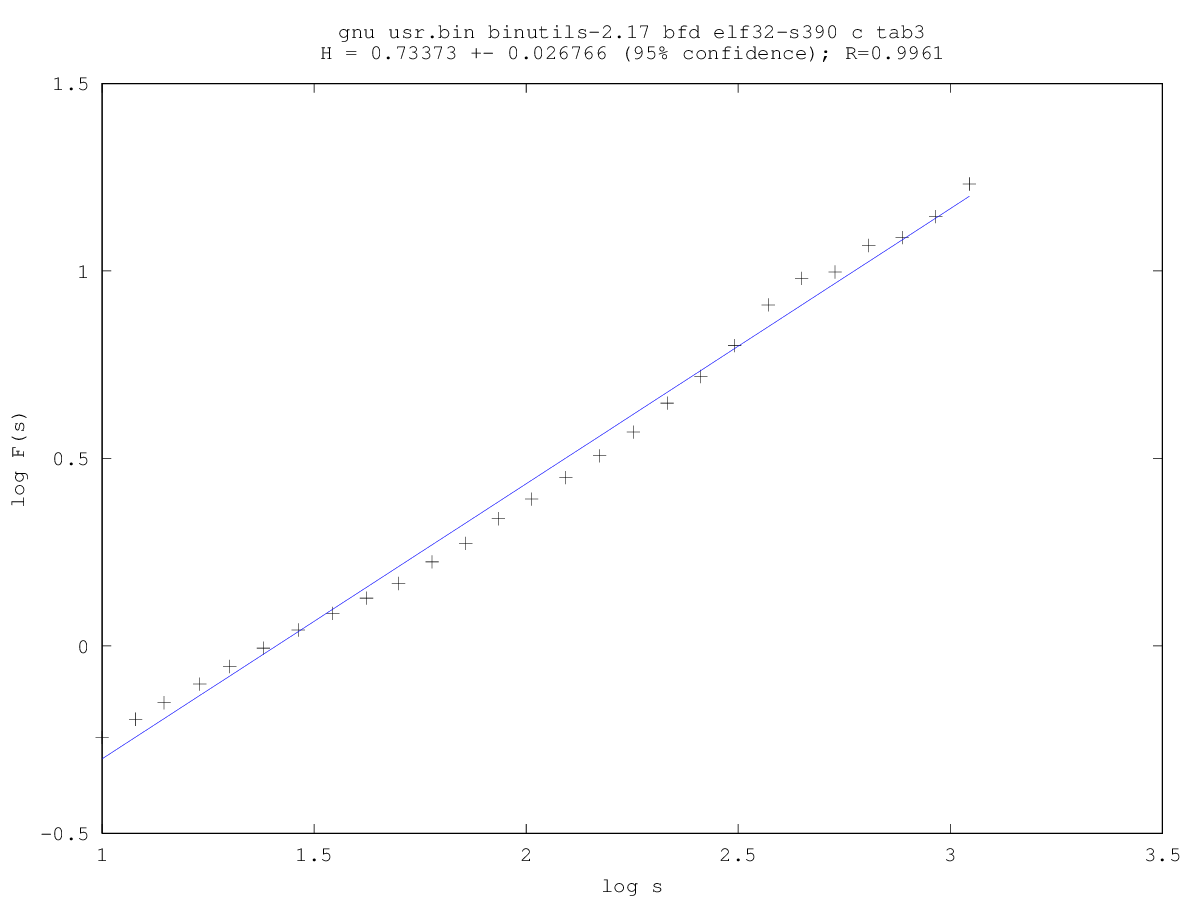
\includegraphics[width=0.8\linewidth]{{fractals/data/gnu_usr.bin_binutils-2.17_bfd_elf32-s390_c_tab3_log_log}.png}
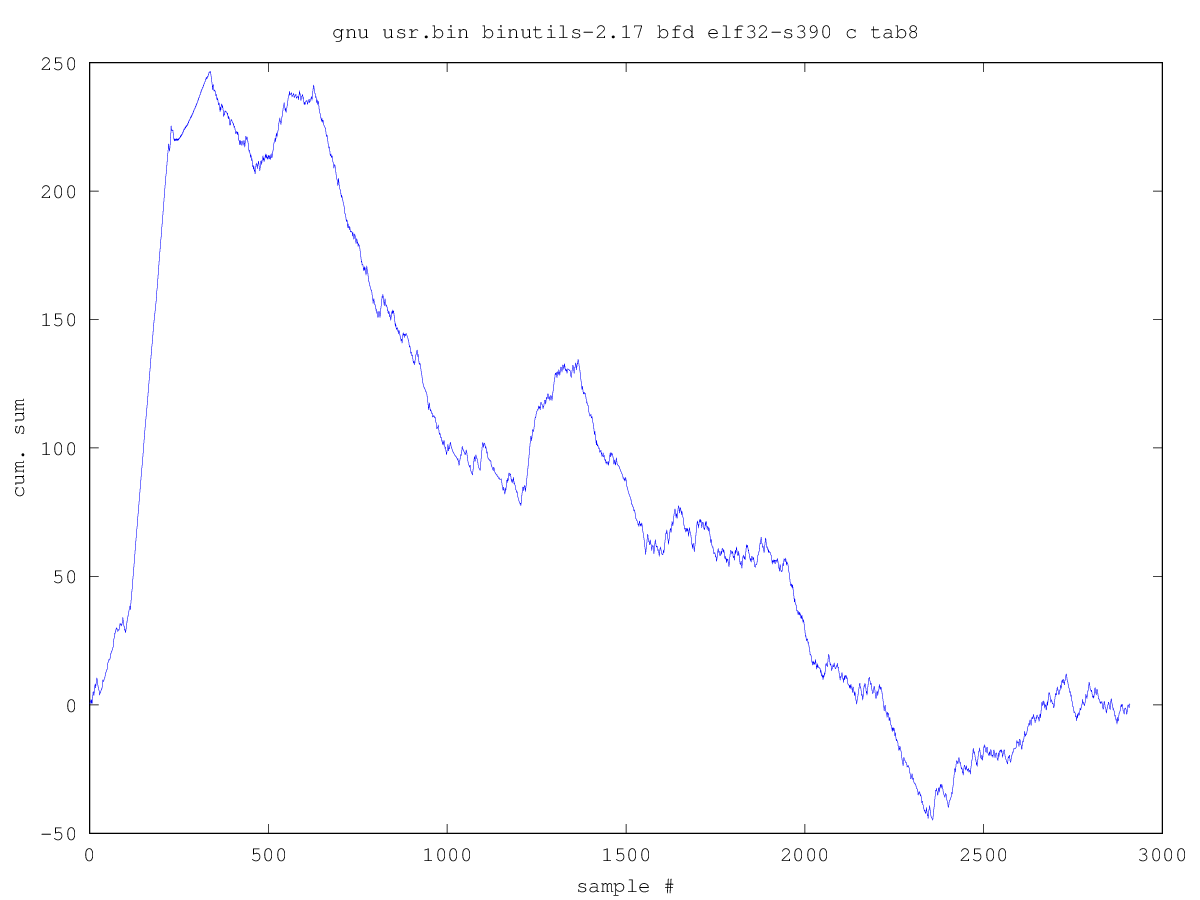
\includegraphics[width=0.8\linewidth]{{fractals/data/gnu_usr.bin_binutils-2.17_bfd_elf32-s390_c_tab8_time_series}.png}
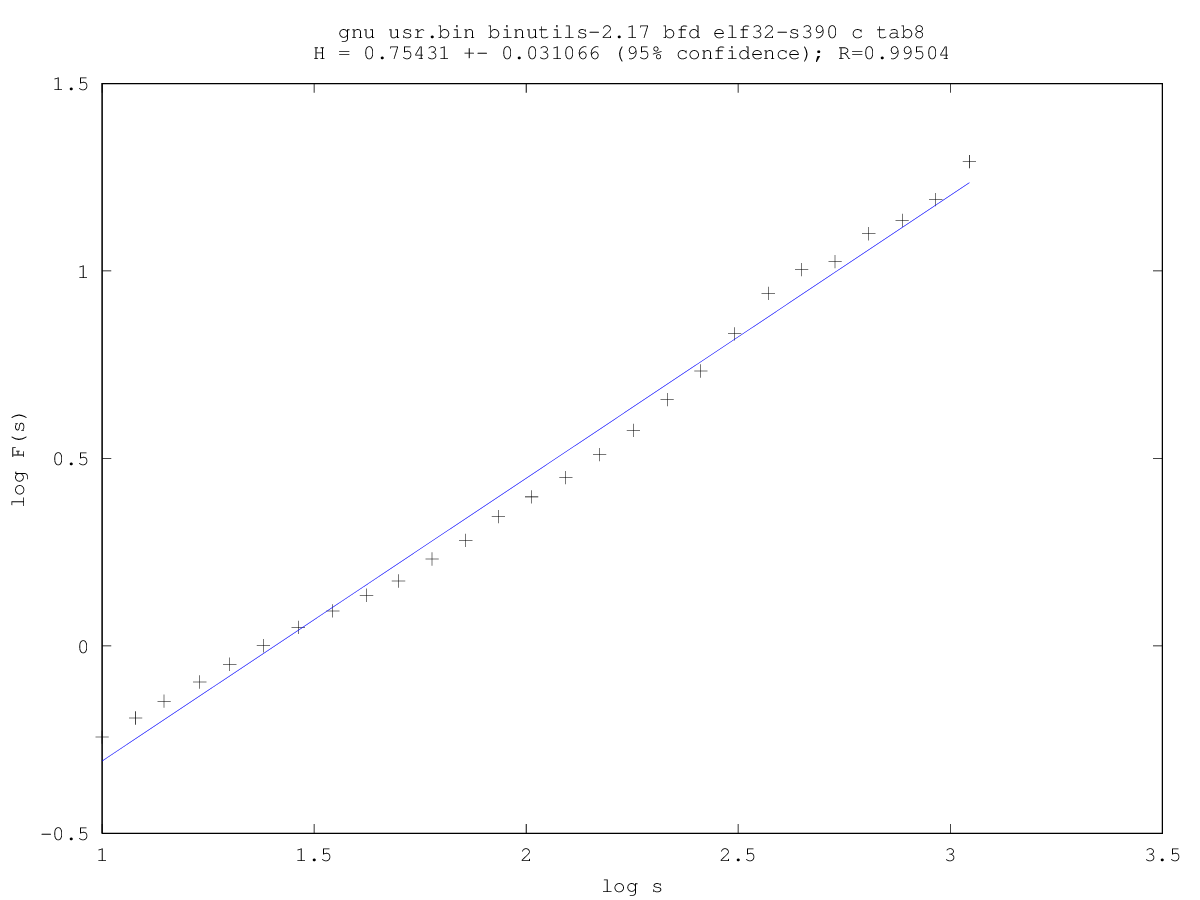
\includegraphics[width=0.8\linewidth]{{fractals/data/gnu_usr.bin_binutils-2.17_bfd_elf32-s390_c_tab8_log_log}.png}
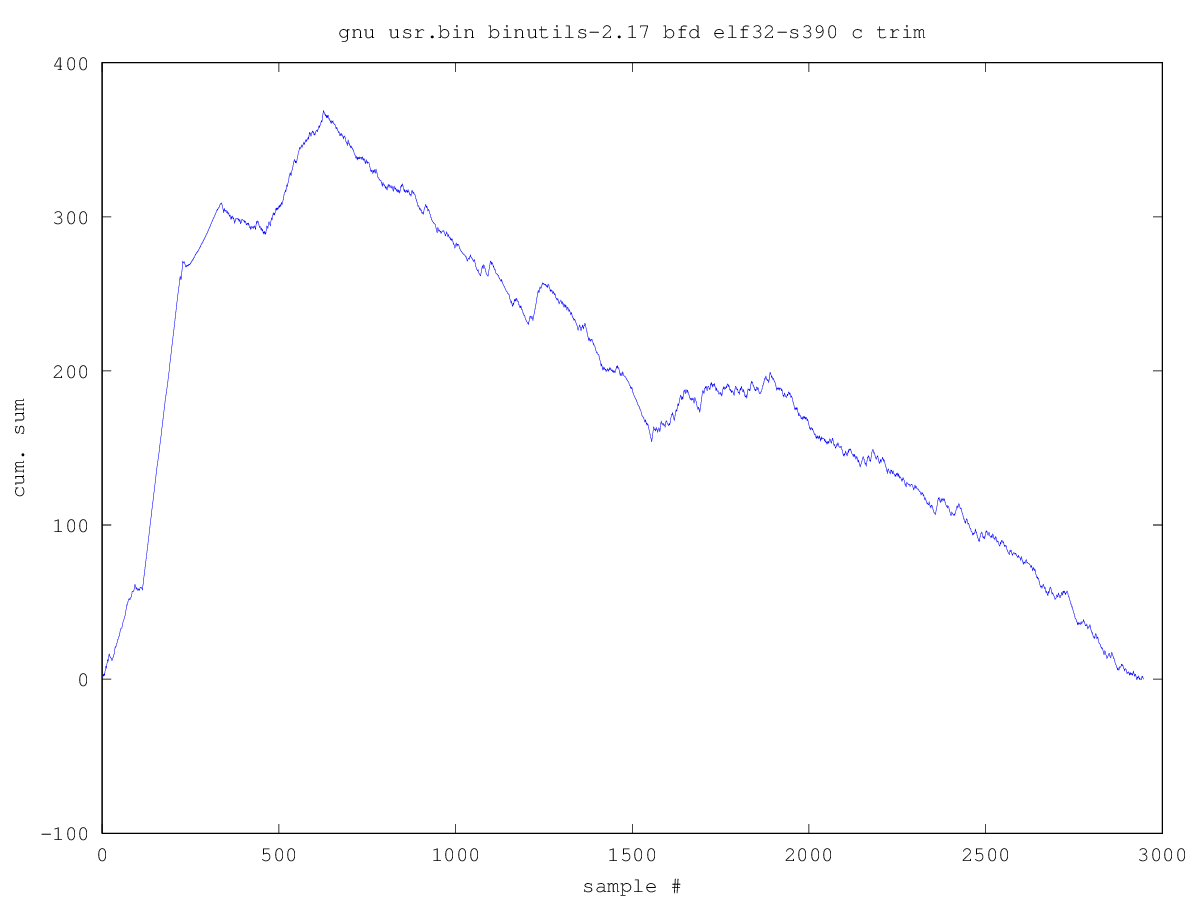
\includegraphics[width=0.8\linewidth]{{fractals/data/gnu_usr.bin_binutils-2.17_bfd_elf32-s390_c_trim_time_series}.png}
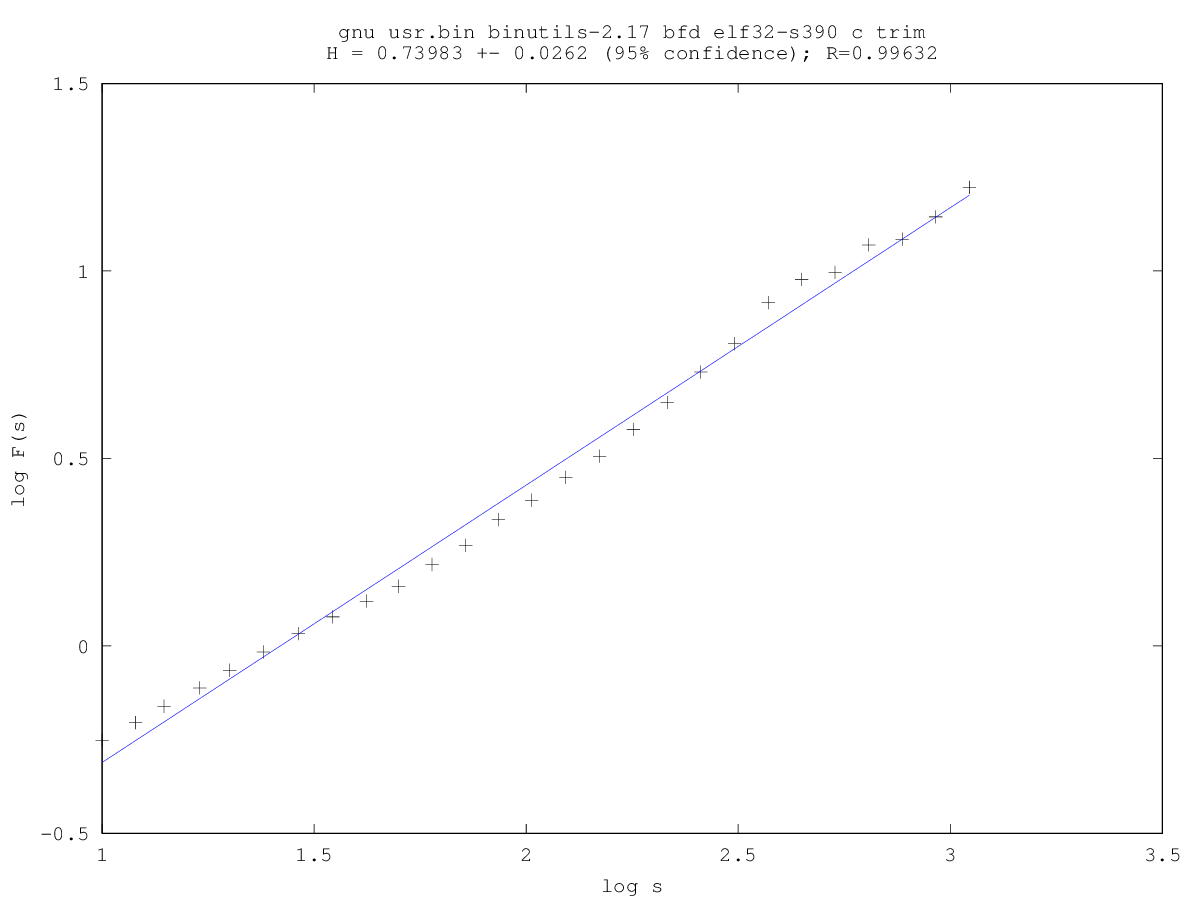
\includegraphics[width=0.8\linewidth]{{fractals/data/gnu_usr.bin_binutils-2.17_bfd_elf32-s390_c_trim_log_log}.png}
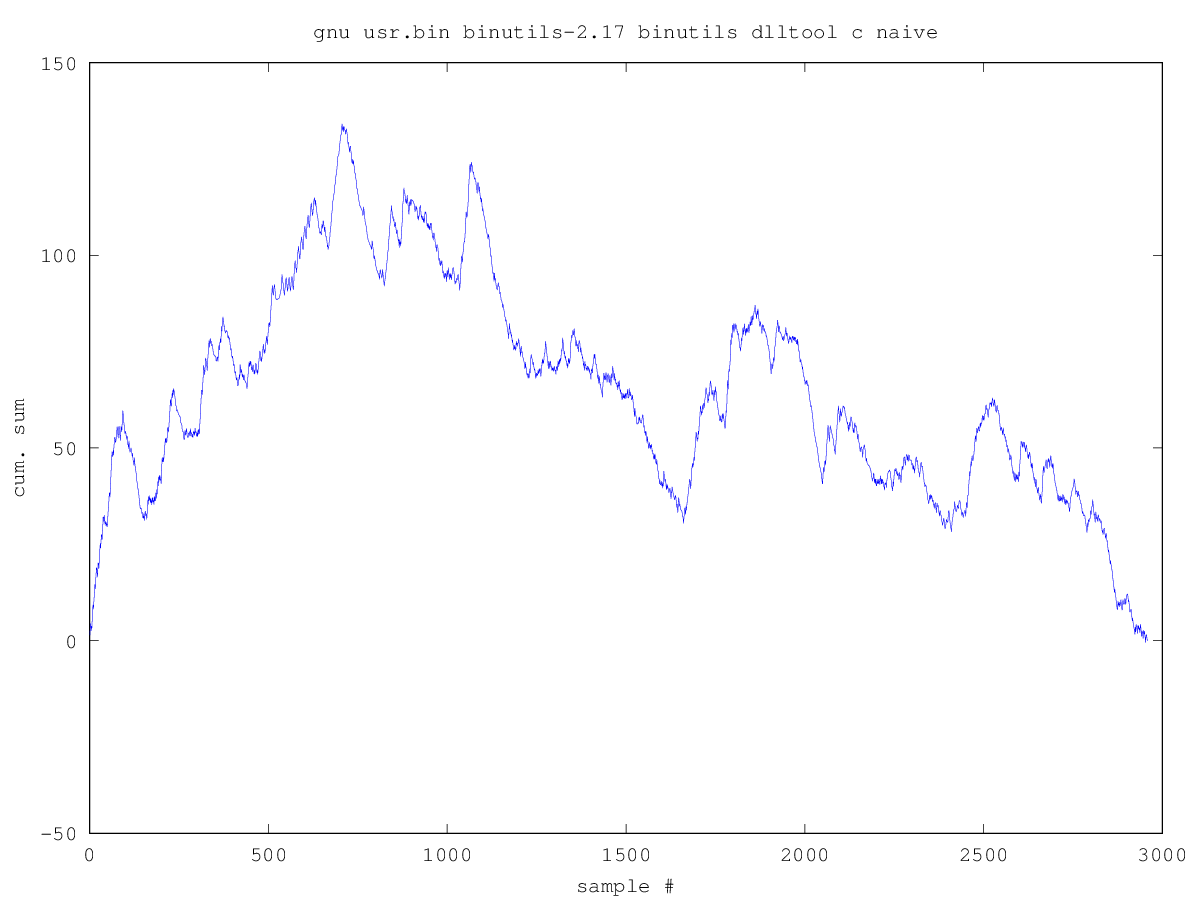
\includegraphics[width=0.8\linewidth]{{fractals/data/gnu_usr.bin_binutils-2.17_binutils_dlltool_c_naive_time_series}.png}
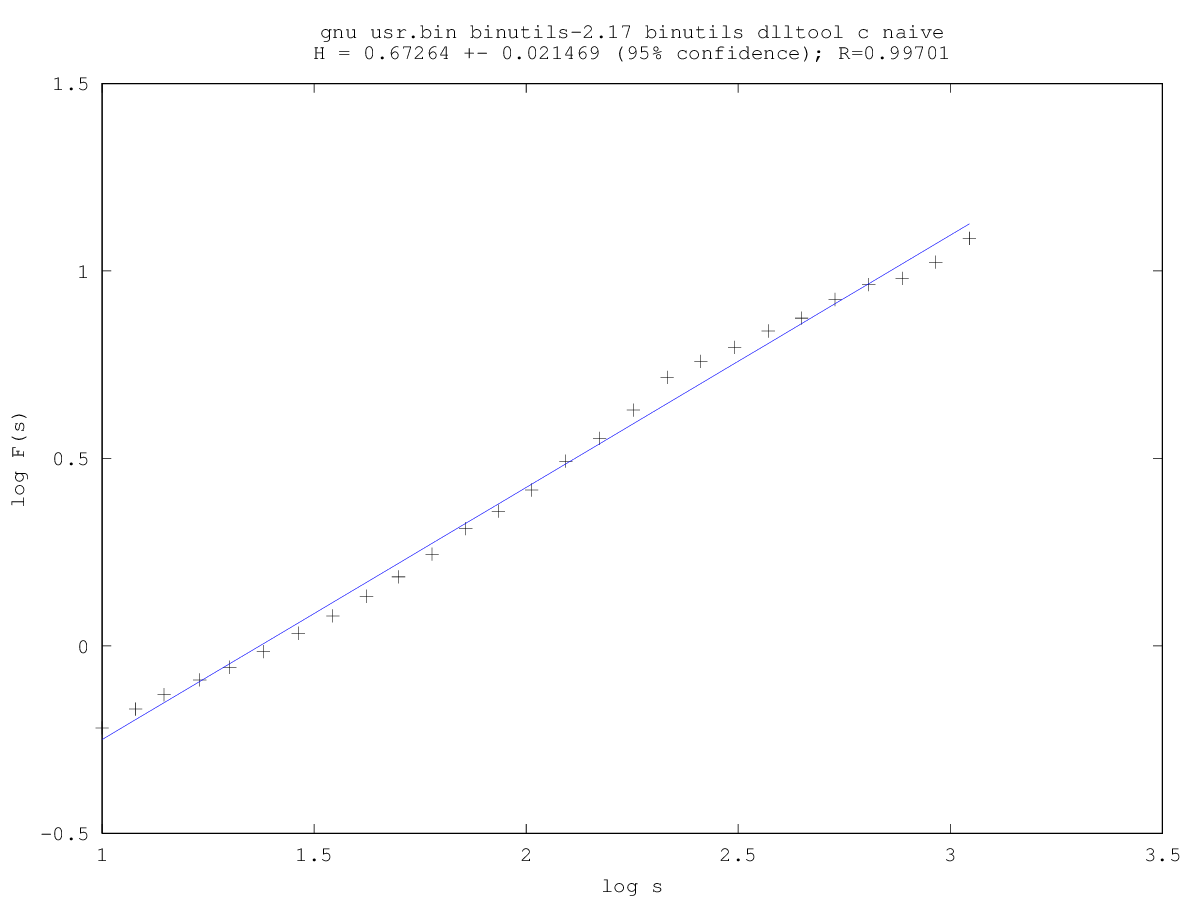
\includegraphics[width=0.8\linewidth]{{fractals/data/gnu_usr.bin_binutils-2.17_binutils_dlltool_c_naive_log_log}.png}
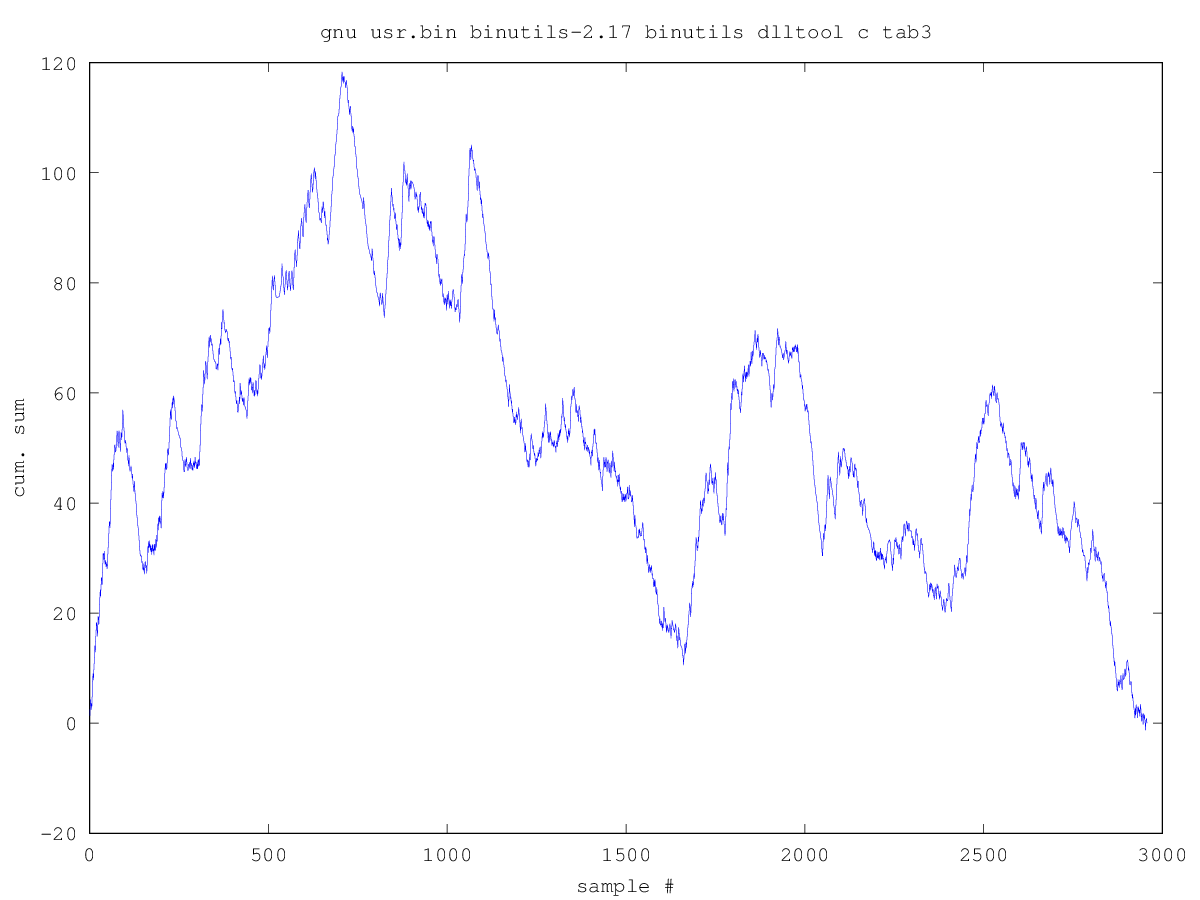
\includegraphics[width=0.8\linewidth]{{fractals/data/gnu_usr.bin_binutils-2.17_binutils_dlltool_c_tab3_time_series}.png}
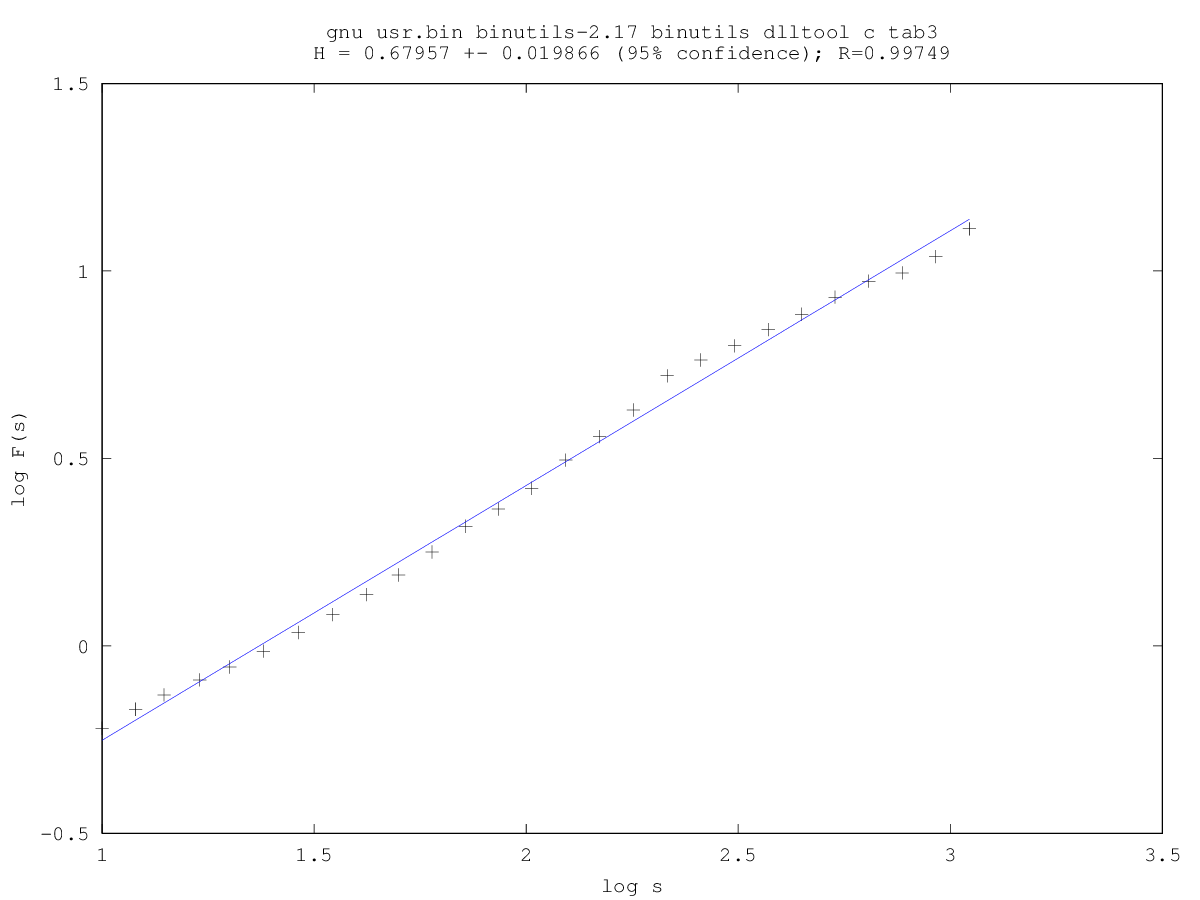
\includegraphics[width=0.8\linewidth]{{fractals/data/gnu_usr.bin_binutils-2.17_binutils_dlltool_c_tab3_log_log}.png}
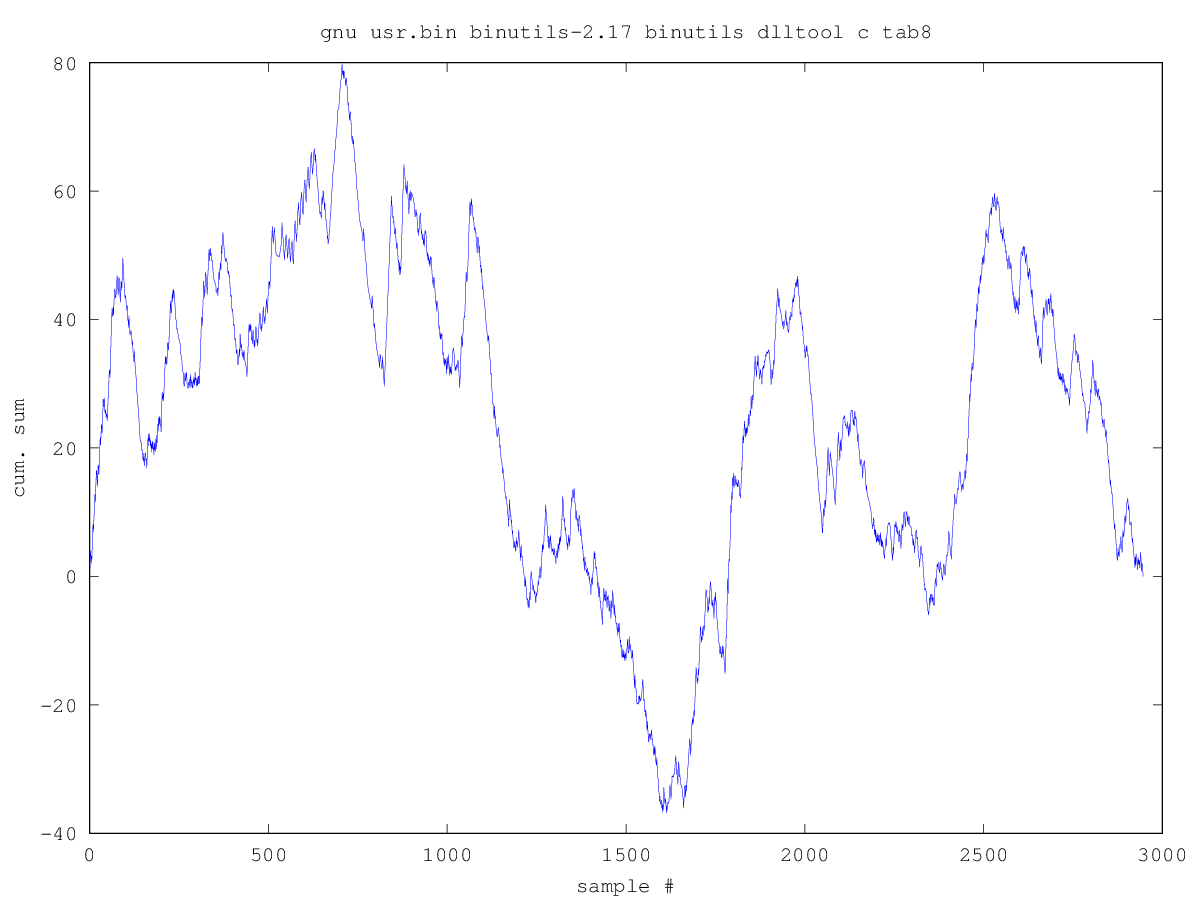
\includegraphics[width=0.8\linewidth]{{fractals/data/gnu_usr.bin_binutils-2.17_binutils_dlltool_c_tab8_time_series}.png}
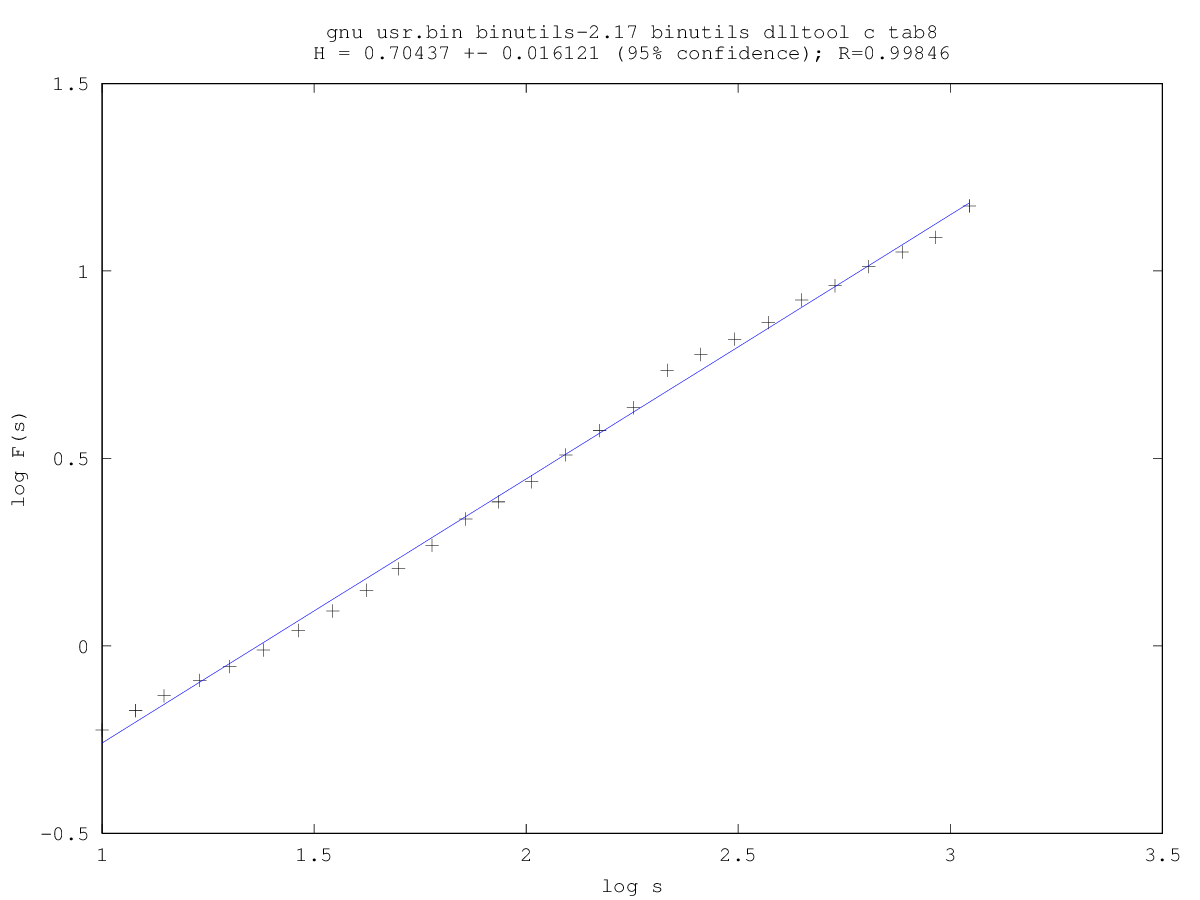
\includegraphics[width=0.8\linewidth]{{fractals/data/gnu_usr.bin_binutils-2.17_binutils_dlltool_c_tab8_log_log}.png}
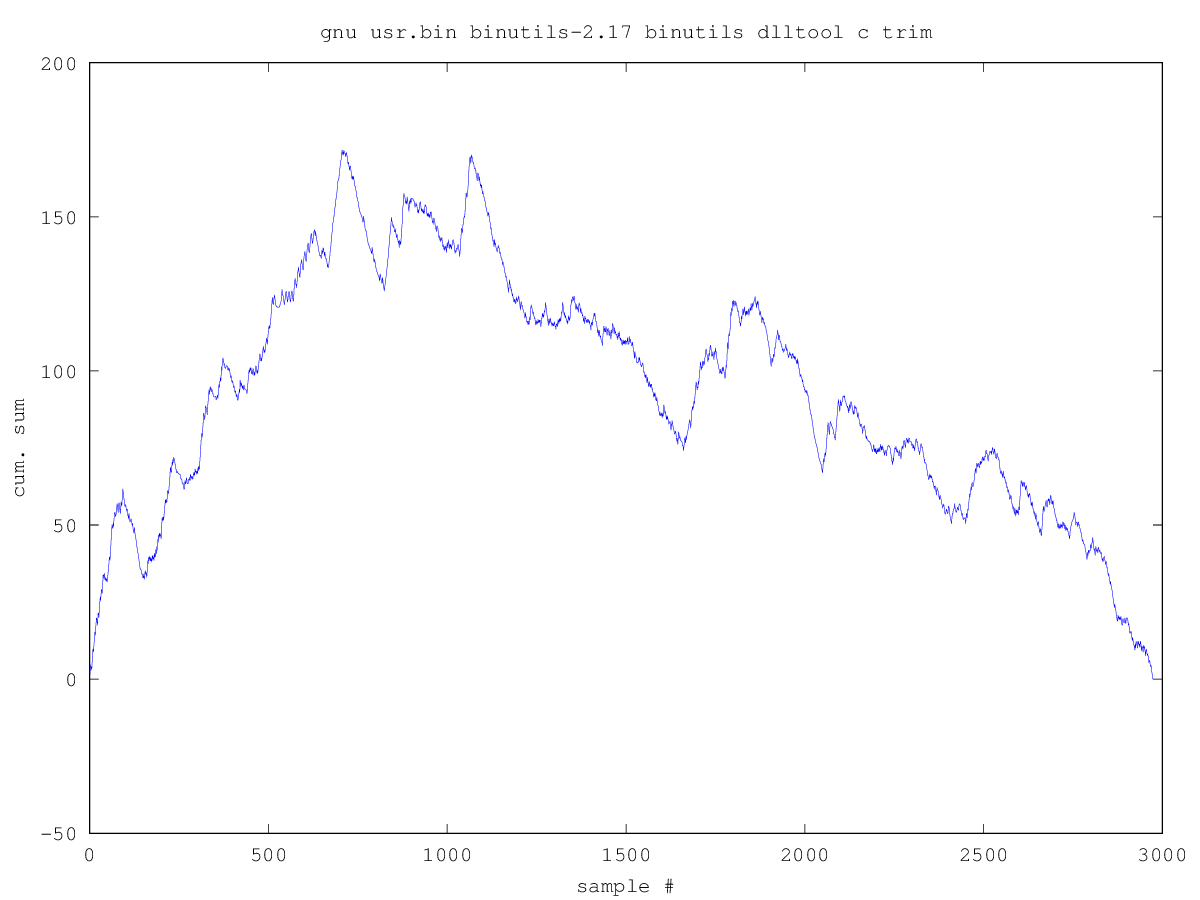
\includegraphics[width=0.8\linewidth]{{fractals/data/gnu_usr.bin_binutils-2.17_binutils_dlltool_c_trim_time_series}.png}
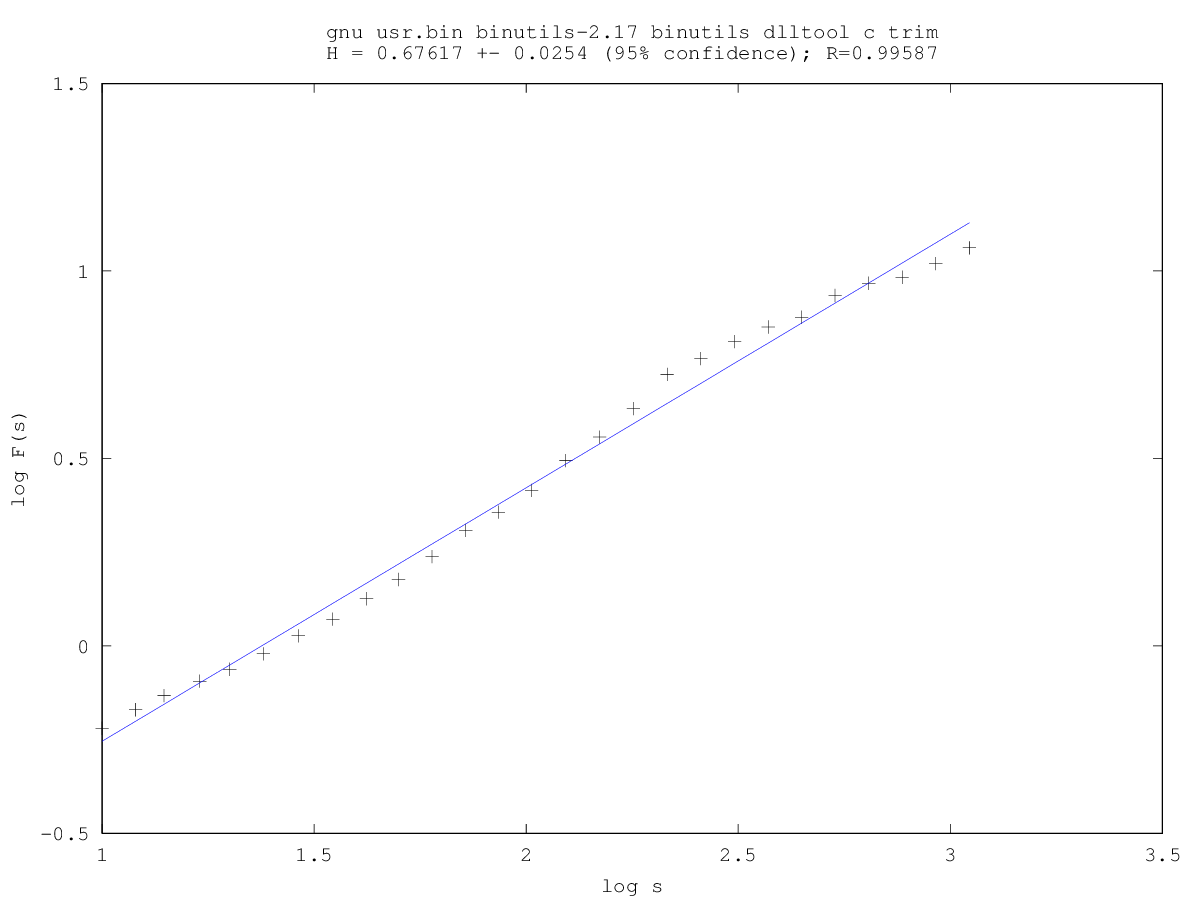
\includegraphics[width=0.8\linewidth]{{fractals/data/gnu_usr.bin_binutils-2.17_binutils_dlltool_c_trim_log_log}.png}
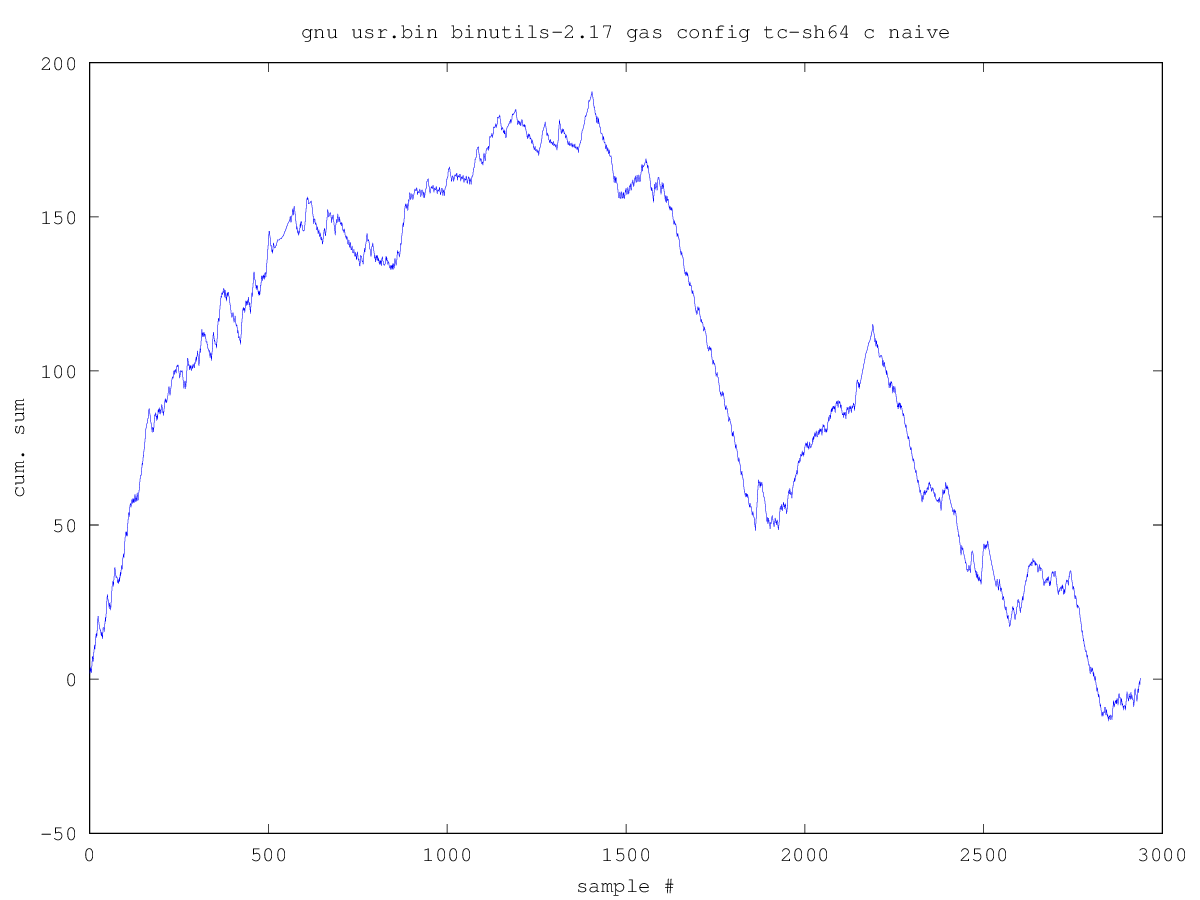
\includegraphics[width=0.8\linewidth]{{fractals/data/gnu_usr.bin_binutils-2.17_gas_config_tc-sh64_c_naive_time_series}.png}
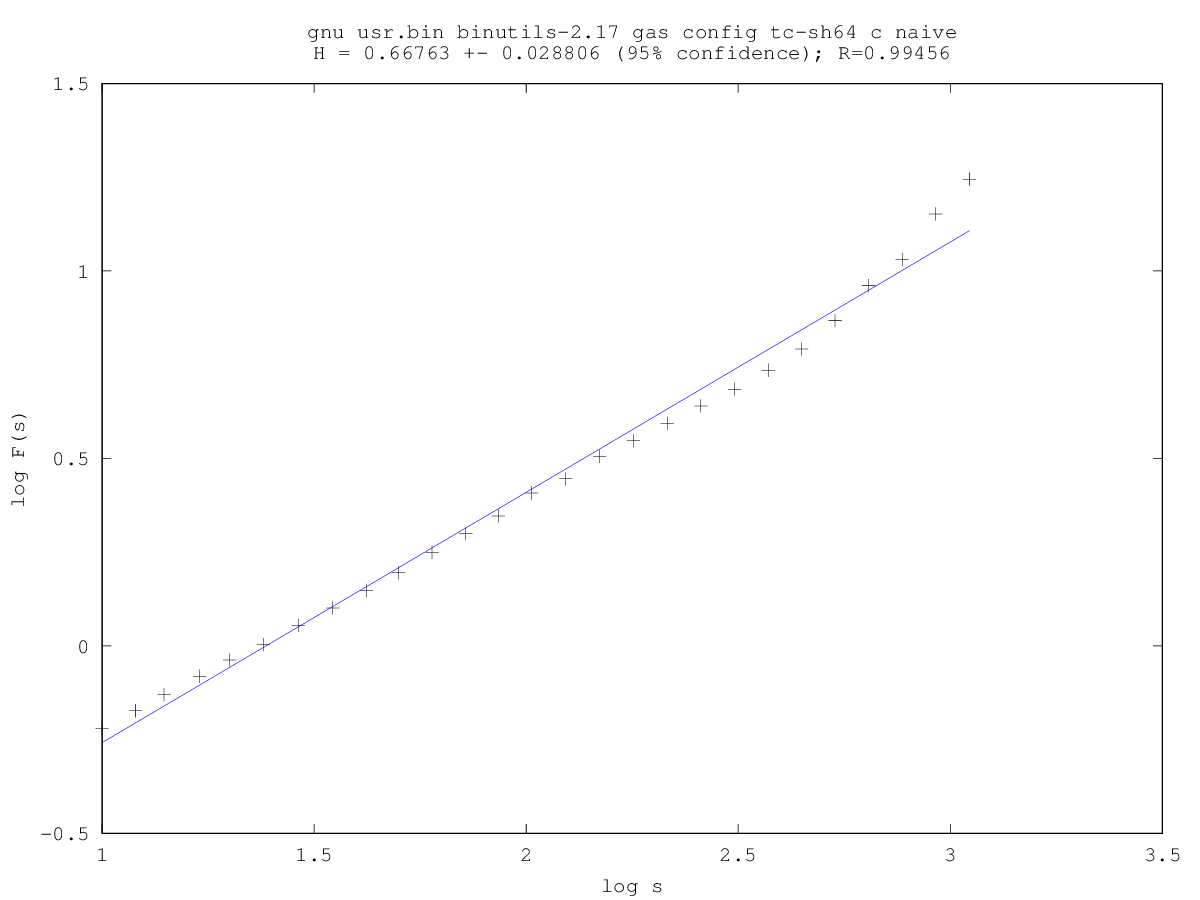
\includegraphics[width=0.8\linewidth]{{fractals/data/gnu_usr.bin_binutils-2.17_gas_config_tc-sh64_c_naive_log_log}.png}
\includegraphics[width=0.8\linewidth]{{fractals/data/gnu_usr.bin_binutils-2.17_gas_config_tc-sh64_c_tab3_time_series}.png}
\includegraphics[width=0.8\linewidth]{{fractals/data/gnu_usr.bin_binutils-2.17_gas_config_tc-sh64_c_tab3_log_log}.png}
\includegraphics[width=0.8\linewidth]{{fractals/data/gnu_usr.bin_binutils-2.17_gas_config_tc-sh64_c_tab8_time_series}.png}
\includegraphics[width=0.8\linewidth]{{fractals/data/gnu_usr.bin_binutils-2.17_gas_config_tc-sh64_c_tab8_log_log}.png}
\includegraphics[width=0.8\linewidth]{{fractals/data/gnu_usr.bin_binutils-2.17_gas_config_tc-sh64_c_trim_time_series}.png}
\includegraphics[width=0.8\linewidth]{{fractals/data/gnu_usr.bin_binutils-2.17_gas_config_tc-sh64_c_trim_log_log}.png}
\includegraphics[width=0.8\linewidth]{{fractals/data/gnu_usr.bin_binutils-2.17_opcodes_xc16x-desc_c_naive_time_series}.png}
\includegraphics[width=0.8\linewidth]{{fractals/data/gnu_usr.bin_binutils-2.17_opcodes_xc16x-desc_c_naive_log_log}.png}
\includegraphics[width=0.8\linewidth]{{fractals/data/gnu_usr.bin_binutils-2.17_opcodes_xc16x-desc_c_tab3_time_series}.png}
\includegraphics[width=0.8\linewidth]{{fractals/data/gnu_usr.bin_binutils-2.17_opcodes_xc16x-desc_c_tab3_log_log}.png}
\includegraphics[width=0.8\linewidth]{{fractals/data/gnu_usr.bin_binutils-2.17_opcodes_xc16x-desc_c_tab8_time_series}.png}
\includegraphics[width=0.8\linewidth]{{fractals/data/gnu_usr.bin_binutils-2.17_opcodes_xc16x-desc_c_tab8_log_log}.png}
\includegraphics[width=0.8\linewidth]{{fractals/data/gnu_usr.bin_binutils-2.17_opcodes_xc16x-desc_c_trim_time_series}.png}
\includegraphics[width=0.8\linewidth]{{fractals/data/gnu_usr.bin_binutils-2.17_opcodes_xc16x-desc_c_trim_log_log}.png}
\includegraphics[width=0.8\linewidth]{{fractals/data/gnu_usr.bin_binutils_binutils_rcparse_c_naive_time_series}.png}
\includegraphics[width=0.8\linewidth]{{fractals/data/gnu_usr.bin_binutils_binutils_rcparse_c_naive_log_log}.png}
\includegraphics[width=0.8\linewidth]{{fractals/data/gnu_usr.bin_binutils_binutils_rcparse_c_tab3_time_series}.png}
\includegraphics[width=0.8\linewidth]{{fractals/data/gnu_usr.bin_binutils_binutils_rcparse_c_tab3_log_log}.png}
\includegraphics[width=0.8\linewidth]{{fractals/data/gnu_usr.bin_binutils_binutils_rcparse_c_tab8_time_series}.png}
\includegraphics[width=0.8\linewidth]{{fractals/data/gnu_usr.bin_binutils_binutils_rcparse_c_tab8_log_log}.png}
\includegraphics[width=0.8\linewidth]{{fractals/data/gnu_usr.bin_binutils_binutils_rcparse_c_trim_time_series}.png}
\includegraphics[width=0.8\linewidth]{{fractals/data/gnu_usr.bin_binutils_binutils_rcparse_c_trim_log_log}.png}
\includegraphics[width=0.8\linewidth]{{fractals/data/gnu_usr.bin_binutils_gas_config_tc-sh64_c_naive_time_series}.png}
\includegraphics[width=0.8\linewidth]{{fractals/data/gnu_usr.bin_binutils_gas_config_tc-sh64_c_naive_log_log}.png}
\includegraphics[width=0.8\linewidth]{{fractals/data/gnu_usr.bin_binutils_gas_config_tc-sh64_c_tab3_time_series}.png}
\includegraphics[width=0.8\linewidth]{{fractals/data/gnu_usr.bin_binutils_gas_config_tc-sh64_c_tab3_log_log}.png}
\includegraphics[width=0.8\linewidth]{{fractals/data/gnu_usr.bin_binutils_gas_config_tc-sh64_c_tab8_time_series}.png}
\includegraphics[width=0.8\linewidth]{{fractals/data/gnu_usr.bin_binutils_gas_config_tc-sh64_c_tab8_log_log}.png}
\includegraphics[width=0.8\linewidth]{{fractals/data/gnu_usr.bin_binutils_gas_config_tc-sh64_c_trim_time_series}.png}
\includegraphics[width=0.8\linewidth]{{fractals/data/gnu_usr.bin_binutils_gas_config_tc-sh64_c_trim_log_log}.png}
\includegraphics[width=0.8\linewidth]{{fractals/data/gnu_usr.bin_gcc_gcc_config_d30v_d30v_c_naive_time_series}.png}
\includegraphics[width=0.8\linewidth]{{fractals/data/gnu_usr.bin_gcc_gcc_config_d30v_d30v_c_naive_log_log}.png}
\includegraphics[width=0.8\linewidth]{{fractals/data/gnu_usr.bin_gcc_gcc_config_d30v_d30v_c_tab3_time_series}.png}
\includegraphics[width=0.8\linewidth]{{fractals/data/gnu_usr.bin_gcc_gcc_config_d30v_d30v_c_tab3_log_log}.png}
\includegraphics[width=0.8\linewidth]{{fractals/data/gnu_usr.bin_gcc_gcc_config_d30v_d30v_c_tab8_time_series}.png}
\includegraphics[width=0.8\linewidth]{{fractals/data/gnu_usr.bin_gcc_gcc_config_d30v_d30v_c_tab8_log_log}.png}
\includegraphics[width=0.8\linewidth]{{fractals/data/gnu_usr.bin_gcc_gcc_config_d30v_d30v_c_trim_time_series}.png}
\includegraphics[width=0.8\linewidth]{{fractals/data/gnu_usr.bin_gcc_gcc_config_d30v_d30v_c_trim_log_log}.png}
\includegraphics[width=0.8\linewidth]{{fractals/data/gnu_usr.bin_gcc_gcc_config_mcore_mcore_c_naive_time_series}.png}
\includegraphics[width=0.8\linewidth]{{fractals/data/gnu_usr.bin_gcc_gcc_config_mcore_mcore_c_naive_log_log}.png}
\includegraphics[width=0.8\linewidth]{{fractals/data/gnu_usr.bin_gcc_gcc_config_mcore_mcore_c_tab3_time_series}.png}
\includegraphics[width=0.8\linewidth]{{fractals/data/gnu_usr.bin_gcc_gcc_config_mcore_mcore_c_tab3_log_log}.png}
\includegraphics[width=0.8\linewidth]{{fractals/data/gnu_usr.bin_gcc_gcc_config_mcore_mcore_c_tab8_time_series}.png}
\includegraphics[width=0.8\linewidth]{{fractals/data/gnu_usr.bin_gcc_gcc_config_mcore_mcore_c_tab8_log_log}.png}
\includegraphics[width=0.8\linewidth]{{fractals/data/gnu_usr.bin_gcc_gcc_config_mcore_mcore_c_trim_time_series}.png}
\includegraphics[width=0.8\linewidth]{{fractals/data/gnu_usr.bin_gcc_gcc_config_mcore_mcore_c_trim_log_log}.png}
\includegraphics[width=0.8\linewidth]{{fractals/data/gnu_usr.bin_gcc_gcc_java_expr_c_naive_time_series}.png}
\includegraphics[width=0.8\linewidth]{{fractals/data/gnu_usr.bin_gcc_gcc_java_expr_c_naive_log_log}.png}
\includegraphics[width=0.8\linewidth]{{fractals/data/gnu_usr.bin_gcc_gcc_java_expr_c_tab3_time_series}.png}
\includegraphics[width=0.8\linewidth]{{fractals/data/gnu_usr.bin_gcc_gcc_java_expr_c_tab3_log_log}.png}
\includegraphics[width=0.8\linewidth]{{fractals/data/gnu_usr.bin_gcc_gcc_java_expr_c_tab8_time_series}.png}
\includegraphics[width=0.8\linewidth]{{fractals/data/gnu_usr.bin_gcc_gcc_java_expr_c_tab8_log_log}.png}
\includegraphics[width=0.8\linewidth]{{fractals/data/gnu_usr.bin_gcc_gcc_java_expr_c_trim_time_series}.png}
\includegraphics[width=0.8\linewidth]{{fractals/data/gnu_usr.bin_gcc_gcc_java_expr_c_trim_log_log}.png}
\includegraphics[width=0.8\linewidth]{{fractals/data/gnu_usr.bin_gcc_gcc_recog_c_naive_time_series}.png}
\includegraphics[width=0.8\linewidth]{{fractals/data/gnu_usr.bin_gcc_gcc_recog_c_naive_log_log}.png}
\includegraphics[width=0.8\linewidth]{{fractals/data/gnu_usr.bin_gcc_gcc_recog_c_tab3_time_series}.png}
\includegraphics[width=0.8\linewidth]{{fractals/data/gnu_usr.bin_gcc_gcc_recog_c_tab3_log_log}.png}
\includegraphics[width=0.8\linewidth]{{fractals/data/gnu_usr.bin_gcc_gcc_recog_c_tab8_time_series}.png}
\includegraphics[width=0.8\linewidth]{{fractals/data/gnu_usr.bin_gcc_gcc_recog_c_tab8_log_log}.png}
\includegraphics[width=0.8\linewidth]{{fractals/data/gnu_usr.bin_gcc_gcc_recog_c_trim_time_series}.png}
\includegraphics[width=0.8\linewidth]{{fractals/data/gnu_usr.bin_gcc_gcc_recog_c_trim_log_log}.png}
\includegraphics[width=0.8\linewidth]{{fractals/data/gnu_usr.bin_perl_hv_c_naive_time_series}.png}
\includegraphics[width=0.8\linewidth]{{fractals/data/gnu_usr.bin_perl_hv_c_naive_log_log}.png}
\includegraphics[width=0.8\linewidth]{{fractals/data/gnu_usr.bin_perl_hv_c_tab3_time_series}.png}
\includegraphics[width=0.8\linewidth]{{fractals/data/gnu_usr.bin_perl_hv_c_tab3_log_log}.png}
\includegraphics[width=0.8\linewidth]{{fractals/data/gnu_usr.bin_perl_hv_c_tab8_time_series}.png}
\includegraphics[width=0.8\linewidth]{{fractals/data/gnu_usr.bin_perl_hv_c_tab8_log_log}.png}
\includegraphics[width=0.8\linewidth]{{fractals/data/gnu_usr.bin_perl_hv_c_trim_time_series}.png}
\includegraphics[width=0.8\linewidth]{{fractals/data/gnu_usr.bin_perl_hv_c_trim_log_log}.png}
\includegraphics[width=0.8\linewidth]{{fractals/data/lib_libpcap_gencode_c_naive_time_series}.png}
\includegraphics[width=0.8\linewidth]{{fractals/data/lib_libpcap_gencode_c_naive_log_log}.png}
\includegraphics[width=0.8\linewidth]{{fractals/data/lib_libpcap_gencode_c_tab3_time_series}.png}
\includegraphics[width=0.8\linewidth]{{fractals/data/lib_libpcap_gencode_c_tab3_log_log}.png}
\includegraphics[width=0.8\linewidth]{{fractals/data/lib_libpcap_gencode_c_tab8_time_series}.png}
\includegraphics[width=0.8\linewidth]{{fractals/data/lib_libpcap_gencode_c_tab8_log_log}.png}
\includegraphics[width=0.8\linewidth]{{fractals/data/lib_libpcap_gencode_c_trim_time_series}.png}
\includegraphics[width=0.8\linewidth]{{fractals/data/lib_libpcap_gencode_c_trim_log_log}.png}
\includegraphics[width=0.8\linewidth]{{fractals/data/sys_arch_arm_arm_pmap7_c_naive_time_series}.png}
\includegraphics[width=0.8\linewidth]{{fractals/data/sys_arch_arm_arm_pmap7_c_naive_log_log}.png}
\includegraphics[width=0.8\linewidth]{{fractals/data/sys_arch_arm_arm_pmap7_c_tab3_time_series}.png}
\includegraphics[width=0.8\linewidth]{{fractals/data/sys_arch_arm_arm_pmap7_c_tab3_log_log}.png}
\includegraphics[width=0.8\linewidth]{{fractals/data/sys_arch_arm_arm_pmap7_c_tab8_time_series}.png}
\includegraphics[width=0.8\linewidth]{{fractals/data/sys_arch_arm_arm_pmap7_c_tab8_log_log}.png}
\includegraphics[width=0.8\linewidth]{{fractals/data/sys_arch_arm_arm_pmap7_c_trim_time_series}.png}
\includegraphics[width=0.8\linewidth]{{fractals/data/sys_arch_arm_arm_pmap7_c_trim_log_log}.png}
\includegraphics[width=0.8\linewidth]{{fractals/data/sys_dev_audio_c_naive_time_series}.png}
\includegraphics[width=0.8\linewidth]{{fractals/data/sys_dev_audio_c_naive_log_log}.png}
\includegraphics[width=0.8\linewidth]{{fractals/data/sys_dev_audio_c_tab3_time_series}.png}
\includegraphics[width=0.8\linewidth]{{fractals/data/sys_dev_audio_c_tab3_log_log}.png}
\includegraphics[width=0.8\linewidth]{{fractals/data/sys_dev_audio_c_tab8_time_series}.png}
\includegraphics[width=0.8\linewidth]{{fractals/data/sys_dev_audio_c_tab8_log_log}.png}
\includegraphics[width=0.8\linewidth]{{fractals/data/sys_dev_audio_c_trim_time_series}.png}
\includegraphics[width=0.8\linewidth]{{fractals/data/sys_dev_audio_c_trim_log_log}.png}
\includegraphics[width=0.8\linewidth]{{fractals/data/sys_dev_ic_mpi_c_naive_time_series}.png}
\includegraphics[width=0.8\linewidth]{{fractals/data/sys_dev_ic_mpi_c_naive_log_log}.png}
\includegraphics[width=0.8\linewidth]{{fractals/data/sys_dev_ic_mpi_c_tab3_time_series}.png}
\includegraphics[width=0.8\linewidth]{{fractals/data/sys_dev_ic_mpi_c_tab3_log_log}.png}
\includegraphics[width=0.8\linewidth]{{fractals/data/sys_dev_ic_mpi_c_tab8_time_series}.png}
\includegraphics[width=0.8\linewidth]{{fractals/data/sys_dev_ic_mpi_c_tab8_log_log}.png}
\includegraphics[width=0.8\linewidth]{{fractals/data/sys_dev_ic_mpi_c_trim_time_series}.png}
\includegraphics[width=0.8\linewidth]{{fractals/data/sys_dev_ic_mpi_c_trim_log_log}.png}
\includegraphics[width=0.8\linewidth]{{fractals/data/sys_dev_isa_gus_c_naive_time_series}.png}
\includegraphics[width=0.8\linewidth]{{fractals/data/sys_dev_isa_gus_c_naive_log_log}.png}
\includegraphics[width=0.8\linewidth]{{fractals/data/sys_dev_isa_gus_c_tab3_time_series}.png}
\includegraphics[width=0.8\linewidth]{{fractals/data/sys_dev_isa_gus_c_tab3_log_log}.png}
\includegraphics[width=0.8\linewidth]{{fractals/data/sys_dev_isa_gus_c_tab8_time_series}.png}
\includegraphics[width=0.8\linewidth]{{fractals/data/sys_dev_isa_gus_c_tab8_log_log}.png}
\includegraphics[width=0.8\linewidth]{{fractals/data/sys_dev_isa_gus_c_trim_time_series}.png}
\includegraphics[width=0.8\linewidth]{{fractals/data/sys_dev_isa_gus_c_trim_log_log}.png}
\includegraphics[width=0.8\linewidth]{{fractals/data/sys_dev_pci_if_oce_c_naive_time_series}.png}
\includegraphics[width=0.8\linewidth]{{fractals/data/sys_dev_pci_if_oce_c_naive_log_log}.png}
\includegraphics[width=0.8\linewidth]{{fractals/data/sys_dev_pci_if_oce_c_tab3_time_series}.png}
\includegraphics[width=0.8\linewidth]{{fractals/data/sys_dev_pci_if_oce_c_tab3_log_log}.png}
\includegraphics[width=0.8\linewidth]{{fractals/data/sys_dev_pci_if_oce_c_tab8_time_series}.png}
\includegraphics[width=0.8\linewidth]{{fractals/data/sys_dev_pci_if_oce_c_tab8_log_log}.png}
\includegraphics[width=0.8\linewidth]{{fractals/data/sys_dev_pci_if_oce_c_trim_time_series}.png}
\includegraphics[width=0.8\linewidth]{{fractals/data/sys_dev_pci_if_oce_c_trim_log_log}.png}
\includegraphics[width=0.8\linewidth]{{fractals/data/sys_dev_pci_if_san_xilinx_c_naive_time_series}.png}
\includegraphics[width=0.8\linewidth]{{fractals/data/sys_dev_pci_if_san_xilinx_c_naive_log_log}.png}
\includegraphics[width=0.8\linewidth]{{fractals/data/sys_dev_pci_if_san_xilinx_c_tab3_time_series}.png}
\includegraphics[width=0.8\linewidth]{{fractals/data/sys_dev_pci_if_san_xilinx_c_tab3_log_log}.png}
\includegraphics[width=0.8\linewidth]{{fractals/data/sys_dev_pci_if_san_xilinx_c_tab8_time_series}.png}
\includegraphics[width=0.8\linewidth]{{fractals/data/sys_dev_pci_if_san_xilinx_c_tab8_log_log}.png}
\includegraphics[width=0.8\linewidth]{{fractals/data/sys_dev_pci_if_san_xilinx_c_trim_time_series}.png}
\includegraphics[width=0.8\linewidth]{{fractals/data/sys_dev_pci_if_san_xilinx_c_trim_log_log}.png}
\includegraphics[width=0.8\linewidth]{{fractals/data/usr.sbin_bgpd_rde_c_naive_time_series}.png}
\includegraphics[width=0.8\linewidth]{{fractals/data/usr.sbin_bgpd_rde_c_naive_log_log}.png}
\includegraphics[width=0.8\linewidth]{{fractals/data/usr.sbin_bgpd_rde_c_tab3_time_series}.png}
\includegraphics[width=0.8\linewidth]{{fractals/data/usr.sbin_bgpd_rde_c_tab3_log_log}.png}
\includegraphics[width=0.8\linewidth]{{fractals/data/usr.sbin_bgpd_rde_c_tab8_time_series}.png}
\includegraphics[width=0.8\linewidth]{{fractals/data/usr.sbin_bgpd_rde_c_tab8_log_log}.png}
\includegraphics[width=0.8\linewidth]{{fractals/data/usr.sbin_bgpd_rde_c_trim_time_series}.png}
\includegraphics[width=0.8\linewidth]{{fractals/data/usr.sbin_bgpd_rde_c_trim_log_log}.png}
\includegraphics[width=0.8\linewidth]{{fractals/data/usr.sbin_nginx_src_http_modules_ngx_http_mp4_module_c_naive_time_series}.png}
\includegraphics[width=0.8\linewidth]{{fractals/data/usr.sbin_nginx_src_http_modules_ngx_http_mp4_module_c_naive_log_log}.png}
\includegraphics[width=0.8\linewidth]{{fractals/data/usr.sbin_nginx_src_http_modules_ngx_http_mp4_module_c_tab3_time_series}.png}
\includegraphics[width=0.8\linewidth]{{fractals/data/usr.sbin_nginx_src_http_modules_ngx_http_mp4_module_c_tab3_log_log}.png}
\includegraphics[width=0.8\linewidth]{{fractals/data/usr.sbin_nginx_src_http_modules_ngx_http_mp4_module_c_tab8_time_series}.png}
\includegraphics[width=0.8\linewidth]{{fractals/data/usr.sbin_nginx_src_http_modules_ngx_http_mp4_module_c_tab8_log_log}.png}
\includegraphics[width=0.8\linewidth]{{fractals/data/usr.sbin_nginx_src_http_modules_ngx_http_mp4_module_c_trim_time_series}.png}
\includegraphics[width=0.8\linewidth]{{fractals/data/usr.sbin_nginx_src_http_modules_ngx_http_mp4_module_c_trim_log_log}.png}

\end{center}

\end{document}